\documentclass[11pt]{article}
\usepackage[utf8]{inputenc}
\usepackage[italian]{babel}
\usepackage{amsmath}
\usepackage{amssymb}
\usepackage{breqn}
\usepackage{amsthm}
\usepackage[small]{caption}

\usepackage{ifpdf}
\setcounter{tocdepth}{5}
\usepackage{nameref}
\usepackage{subcaption}
\usepackage[backend = bibtex]{biblatex}
\bibliography{include/bibliografia}


\ifpdf 
    \usepackage[pdftex]{graphicx}   % to include graphics
    \pdfcompresslevel=9 
    \usepackage[pdftex,     % sets up hyperref to use pdftex driver
            plainpages=false,   % allows page i and 1 to exist in the same document
            breaklinks=true,    % link texts can be broken at the end of line
            colorlinks=true,
            linkcolor=blue,
            pdftitle=Appunti di Machine Learning
            pdfauthor=Maurizio Dimatteo
           ]{hyperref} 
    \usepackage{thumbpdf}
\else 
    \usepackage{graphicx}       % to include graphics
    \usepackage[hypertexnames=false]{hyperref}       % to simplify the use of \href
\fi 

\usepackage[usenames,dvipsnames]{color}
\usepackage{listings}

\DeclareMathOperator*{\argmin}{arg\!\min}
\DeclareMathOperator*{\argmax}{arg\!\max}
\DeclareMathOperator*{\cov}{Cov}
\DeclareMathOperator*{\sign}{sign}

\theoremstyle{definition}
\newtheorem*{esempio}{Esempio}


\title{Appunti di Machine Learning}
\author{Maurizio Dimatteo \\ \href{mailto:dimatteomaurizio@gmail.com}{\small dimatteomaurizio@gmail.com}}
\date{\today}

\begin{document}

\lstset{ 
  language=R,                     % the language of the code
  basicstyle=\scriptsize\ttfamily, % the size of the fonts that are used for the code
  %numbers=left,                   % where to put the line-numbers
  %numberstyle=\tiny\color{Blue},  % the style that is used for the line-numbers
  %stepnumber=1,                   % the step between two line-numbers. If it's 1, each line
                                  % will be numbered
  %numbersep=5pt,                  % how far the line-numbers are from the code
  backgroundcolor=\color{white},  % choose the background color. You must add \usepackage{color}
  showspaces=false,               % show spaces adding particular underscores
  showstringspaces=false,         % underline spaces within strings
  showtabs=false,                 % show tabs within strings adding particular underscores
  frame=single,                   % adds a frame around the code
  rulecolor=\color{black},        % if not set, the frame-color may be changed on line-breaks within not-black text (e.g. commens (green here))
  tabsize=2,                      % sets default tabsize to 2 spaces
  captionpos=b,                   % sets the caption-position to bottom
  breaklines=true,                % sets automatic line breaking
  breakatwhitespace=false,        % sets if automatic breaks should only happen at whitespace
    keywordstyle=\color{RoyalBlue},      % keyword style
  commentstyle=\color{YellowGreen},   % comment style
  stringstyle=\color{ForestGreen}      % string literal style
} 

\maketitle
\begingroup
\hypersetup{linkcolor=black}
\tableofcontents
\endgroup

\section*{Premesse}
\begin{itemize}
\item Ho scritto questi appunti (non sono sbobinature) durante le lezioni di \emph{Machine Learning }tenute dall'ing.\@ Ostuni nell'a.a.\@ 2013/2014. 

\item Ho fatto del mio meglio, ma non posso garantire che siano privi di imprecisioni teoriche e strafalcioni. Se ne trovi scrivimi all'indirizzo email in copertina.

\item Il loro scopo principale è coprire gli argomenti che non sono trattati sul libro di riferimento del corso~\cite{AIMA} o che sono trattati diversamente da come ci sono stati esposti a lezione. Per questo motivo gli appunti non sono esaustivi e per alcuni argomenti rimando direttamente al libro. Se hai voglia di completare le parti mancanti scrivimi tramite email.

\item Questa dispensa è complementare alle lezioni in aula ed alle slide dell'ing.\@  Ostuni. Studiarla non è condizione sufficiente (e tantomeno necessaria) per il superamento dell'esame.

\item Né l'ing.\@  Ostuni, né il prof.\@  Di Noia hanno rivisto, corretto o autorizzato ufficialmente questi appunti.
\end{itemize}

\section*{Changelog}

\begin{itemize}
    
    \item TBD
    \begin{itemize}
    \item Aggiunto: \nameref{scelta-p};
    \item Modificato: \nameref{sec:k-means}.
    \end{itemize}

     \item 2014/04/19
     \begin{itemize}
     \item Modificato: \nameref{sec:funzione_costo_logistica}.
     \end{itemize}
     
    
    \item 2014/04/15 \begin{itemize}
        \item Aggiunto: \nameref{sec:dim_log_regr};
        \item Ampliato: \nameref{sec:regolarizzazione_l2};
        \item Altre correzioni minori.
     \end{itemize}
     
     \item 2014/03/17: Prima pubblicazione.
    
\end{itemize}


\section{Introduzione}

\subsection{Ragionamento deduttivo e induttivo}
\
Si dice \emph{ragionamento deduttivo} il processo per cui, partendo dalla conoscenza generale del fenomeno, si arriva a conclusioni specifiche. Con riferimento ad una \emph{blackbox} è come conoscere la funzione di trasferimento ed applicarla agli ingressi per ricavarne le uscite.

Il \emph{ragionamento induttivo}, invece, si basa sull'osservazione di esempi specifici per ricavare una regola generale che giustifichi gli esempi visti. È equivalente ad osservare ingressi ed uscite di una \emph{blackbox} ed individuare la migliore approssimazione della funziona di trasferimento.

\paragraph{Esempio}
\begin{itemize}
  \item  Ragionamento deduttivo:
    \begin{itemize}
      \item assioma generale: tutti i cani hanno quattro zampe, una coda ed abbaiano;
    \item conclusione specifica: questo che ho davanti è un cane (perché ha quattro zampe, una coda ed abbaia).
    \end{itemize}
  \item  Ragionamento induttivo:
  \begin{itemize}
  \item esempio specifico: questi animali hanno quattro zampe, una coda ed abbaiano;  \item descrizione generale: deve esistere una categoria di animali con queste caratteristiche (chiamati ``cani'').
  \end{itemize}
\end{itemize}

\subsection{Apprendimento supervisionato e non supervisionato}

\subsubsection{Supervisionato}
Dato un \emph{traininig set} in cui ciascuna istanza è costituita da un vettore di \emph{feature} ($\mathbf{x}$) ed il corrispondente \emph{output} ($y$), l'apprendimento supervisionato consiste nell'individuare la migliore funzione  $h(x)$ (detta ``ipotesi'') che approssima la funzione \emph{target} $f(x)$ (sconosciuta) tale che $y = f(x) \cong h(x)$ anche per valori esterni al \emph{training set}.

Si possono individuare due categorie di algoritmi supervisionati:
\begin{itemize}
\item algoritmi di regressione;
\item algoritmi di classificazione.
\end{itemize}


\paragraph{Algoritmi di regressione} Forniscono un \emph{output} numerico e tentano di approssimare una funzione non nota. Ad esempio potremmo istruire una macchina per emulare il comportamento di una funzione matematica $f(x)$. L'\emph{output} $y=h(x)$ sarà numerico e rappresenterà una stima di $f(x)$.

\paragraph{Algoritmi di classificazione} Forniscono un \emph{output} qualitativo, specificano cioè la classe di appartenenza di ciascun campione in ingresso. Ad esempio un classificatore binario potrebbe essere addestrato con dati relativi ad altezza e peso di un certo numero di uomini e di donne. In fase di predizione, ricevuti in ingresso altezza e peso di una persona, l'uscita del classificatore sarà 1 o 0 a seconda che altezza e peso siano più consoni ad una donna o ad un uomo.

\subsubsection{Non supervisionato}
In questa categoria di algoritmi non abbiamo a disposizione le uscite corrispondenti a ciascun vettore di \emph{feature}. Lo scopo della macchina è estrapolare delle informazioni significative dagli ingressi. A tal proposito si possono perseguire i seguenti due scopi principali.

\paragraph{Clusterizzazione}
Consiste nell'individuare gruppi di vettori di \emph{input} con caratteristiche comuni. Ad esempio fornendo altezza e peso di 100 persone, tramite un algoritmo di clusterizzazione potremmo individuare una suddivisione dell'insieme dei campioni in due \emph{cluster}: adulti e bambini, oppure uomini e donne. A priori, però, non conosciamo per ciascun vettore di \emph{feature} la corrispondente classe di appartenenza.

\paragraph{Dimensionality reduction}
Consiste nell'individuare quali \emph{feature} sono poco rilevanti ai fini della classificazione in modo tale da poterle trascurare e ridurre le dimensioni del problema.

\subsection{Scelta della migliore ipotesi}

Essa idealmente dovrebbe:
\begin{itemize}
  \item minimizzare l'errore commesso sul \emph{training set};
  \item essere capace di generalizzare l'andamento del fenomeno, ovvero predire correttamente anche \emph{output} non noti relativi ad ingressi mai visti durante l'addestramento.
  \end{itemize}
I due obiettivi sono spesso incompatibili, per cui occorre trovare il giusto compromesso ed evitare \emph{underfitting} ed \emph{overfitting} (\autoref{sec:overunderfitting}).

\subsubsection{Rasoio di Occam}
Quella del Rasoio di Occam è una regola di massima che ci suggerisce come scegliere l'ipotesi più opportuna. Preso un insieme di ipotesi di grado massimo $k$, assumendo che rappresentino tutte adeguatamente il modello, il principio del Rasoio di Occam (che ha origini lontane dall'AI e dalla scienza) ci suggerisce di optare per quella più semplice. È ragionevole pensare che l'ipotesi più semplice sia quella di grado minore. Specifichiamo che un'ipotesi rappresenta adeguatamente un modello quando è consistente con l'insieme di esempi forniti, cioè quando si accorda con tutti i dati osservati\footnote{AIMA - Paragrafo 18.2}. Quindi nella scelta del modello occorre cercare un buon compromesso tra consistenza e bassa complessità dell'ipotesi.

\subsection{Modelli discriminativi e generativi}
Un'ulteriore classificazione dei modelli è tra \emph{discriminativi} e \emph{generativi}.

\subsubsection{Discriminativi}

Si tratta di modelli che, in seguito all'addestramento su un \emph{training set}, quando ricevono in ingresso un vettore $\mathbf{x}$, sono in grado di valutare quale tra le possibili uscite è quella più probabile (ad esempio qual è la classe di appartenenza più probabile del campione ricevuto). Hanno lo scopo di stimare la probabilità condizionata $p(y|\mathbf{x})$, cioè la probabilità che, dato l'ingresso $\mathbf{x}$, esso generi l'uscita $y$ (dove $y$ potrebbe rappresentare la possibile classe del campione).

\subsubsection{Generativi}
Contrariamente ai precedenti, stimano la probabilità congiunta $p(\mathbf{x},y)$. A partire da ciascun possibile \emph{output} viene generato un modello probabilistico degli \emph{input} ad esso associato. Ciò consente di generare, dato un possibile \emph{output}, un \emph{input} che con buona probabilità potrà essere associato ad esso.
\section{Algoritmi di regressione lineari}

\subsection{Regressione semplice lineare}
Si chiama semplice perché prevede ingressi scalari (e non vettori di \emph{feature}). È lineare perché, dato un \emph{training set} di coppie $(x_i, y_i)$, cerca la miglior retta che ne approssima l'andamento.

La generica ipotesi ha espressione:
\begin{equation*}
 h(x) = \theta_0 + \theta_1 x
\end{equation*}
dove:
\begin{itemize}
  \item $\theta_0$ prende il nome di \emph{bias} e rappresenta l'intercetta con l'asse delle $y$;
  \item $\theta_1$ è il coefficiente angolare della retta desiderata.
\end{itemize}
Lo scopo della fase di \emph{training} è individuare i valori ottimi dei parametri $\theta_i$ (vedremo a breve cosa si intende per valori ottimi).

\subsection{Regressione multipla lineare}
È simile alla regressione semplice lineare, ma gli ingressi sono vettori di \emph{feature}.  Dunque non cerchiamo una retta, ma un iperpiano separatore, dalla generica espressione:
\begin{equation*}
  h(x) = \theta_0 + \sum_{i=1}^n \theta_i x_i.
\end{equation*}
Introducendo $x_0=1$ possiamo riscrivere la precedente come segue
\begin{equation*}
  h(x) = \sum_{i=0}^n \theta_i x_i = \theta^T \mathbf{x}
\end{equation*}
dove 
\begin{itemize}
  \item $\theta = {(\theta_0, \theta_1, \dots, \theta_n)}^T$ rappresenta il vettore dei parametri da apprendere durante la fase di addestramento;
  \item $n$ rappresenta la dimensione degli ingressi, cioè il numero di \emph{feature}. Notiamo che per $n$ ingressi occorre apprendere $n+1$ parametri $\theta_i$.
\end{itemize}

\subsubsection{Funzione costo}
Per individuare i valori ottimi dei $\theta_i$ costruiamo una funzione costo $J(\theta)$. Essa deve tener conto della differenza tra i valori di \emph{output} forniti dal \emph{training set} e gli stessi valori calcolati tramite l'ipotesi $h(x)$. Avrà quindi questa espressione:
\begin{equation}\label{eqJ_theta_semplice}
  J(\theta) = \frac{1}{2m} \sum_{i=1}^m (h_\theta(\mathbf{x^{(i)}})-y^{(i)})^2
\end{equation}
dove:
\begin{itemize}
  \item $m$ è il numero di istanze del \emph{training set};
  \item $\frac{1}{2m}$ è un fattore di normalizzazione, il coefficiente $2$ viene introdotto per semplificare le derivate parziali (vedi \autoref{sec:gradiente});
  \item $(h_\theta(\mathbf{x^{(i)}})-y^{(i)})$ è l'errore di predizione sul campione \emph{i-esimo}, calcolato come differenza tra l'\emph{output} stimato dal modello e quello letto dal \emph{training set}.
\end{itemize}
Elevando al quadrato e sommando ciascun errore si ottiene una funzione $J(\theta)$ quadratica  facilmente (e sicuramente) minimizzabile. Lo scopo della fase di apprendimento è quindi individuare per quali $\theta$ la funzione costo è minima:
\begin{equation*}
  \theta_{min} = \argmin_\theta( J(\theta)).
\end{equation*}

\subsection{Metodo delle equazioni normali}
Un primo approccio alla minimizzazione della funzione costo è quello analitico.
Definiamo innanzitutto una matrice $\mathbf{X}$ di dimensioni $m \times (n+1)$ in cui ciascuna riga rappresenta un ingresso nel \emph{training set}. Definiamo, inoltre, un vettore colonna $\mathbf{y}$ di $m$ elementi, ciascuno dei quali rappresenta l'uscita associata all'ingresso \emph{i-esimo} (nonché riga \emph{i-esima} di $\mathbf{X}$):

\begin{equation*}
\mathbf{X} = \begin{bmatrix}
 \mathbf{x^{(1)T}}\\
 \mathbf{x^{(2)T}}\\
 \vdots \\
  \mathbf{x^{(i)T}}\\
  \vdots \\
   \mathbf{x^{(m)T}}\\
\end{bmatrix} \qquad
\mathbf{y} = \begin{bmatrix}
 y^{(1)}\\
 y^{(2)}\\
 \vdots \\
 y^{(i)}\\
  \vdots \\
 y^{(m)}\\
\end{bmatrix}
\end{equation*}
La funzione costo può essere riscritta sotto forma di prodotto tra matrici:
\begin{equation*}
J(\theta) = \frac{1}{2} (\mathbf{X}\theta - \mathbf{y})^T (\mathbf{X}\theta - \mathbf{y}).
\end{equation*}
Cerchiamo il punto di minimo annullandone il gradiente:
\begin{equation*}
\nabla J(\theta) = \mathbf{X}^T\mathbf{X}\theta - \mathbf{X}^T \mathbf{y} = 0
\end{equation*}
da cui si ricava che
\begin{equation*}
\hat\theta = (\mathbf{X}^T\mathbf{X})^{-1} \mathbf{X}^T \mathbf{y}.
\end{equation*}
Questo metodo richiede il calcolo dell'inversa di $(\mathbf{X}^T\mathbf{X})$, di dimensioni $(n+1) \times (n+1)$. Quando il numero di \emph{feature} è piuttosto grande, questo calcolo diventa troppo costoso: tipicamente la complessità computazionale del calcolo dell'inversa è $\mathcal{O}(n^3)$ e questo può rendere il metodo delle equazioni normali anche più lento di metodi iterativi come la discesa a gradiente\footnote{\href{http://www.youtube.com/watch?v=B3vseKmgi8E}{{Coursera, Machine Learning (Andrew Ng), Lezione 4.6}}}. Per tale motivo, quando il numero di \emph{feature} è almeno nell'ordine di $10^5$, si preferiscono metodi numerici come quello della discesa del gradiente che analizzeremo in seguito. Il metodo delle equazioni normali, tuttavia, essendo analitico non richiede la determinazione empirica di alcun parametro (contrariamente a quanto accade con il \emph{learning rate} nella discesa a gradiente) e non è necessario effettuare alcun tipo di \emph{feature scaling} (di cui parleremo in \autoref{feature_scaling}).

In ultimo, consideriamo il caso in cui $\mathbf{X}^T\mathbf{X}$ non sia invertibile. Questo si verifica raramente, e se accade le cause più probabili sono due\footnote{\href{http://www.youtube.com/watch?v=0TMfGA3zQFQ}{Coursera, Machine Learning (Andrew Ng), Lezione 4.7}}:
\begin{itemize}
\item ci sono 2 o più \emph{feature} linearmente dipendenti, per cui è sufficiente eliminarle tutte tranne una;
\item il numero di esempi di addestramento è troppo basso rispetto al numero di \emph{feature}. Questo problema può essere risolto eliminando alcune \emph{feature} tramite tecniche di \emph{feature selection} oppure adottando tecniche di regolarizzazione.
\end{itemize}


\subsubsection{Dimostrazione}
Deriviamo ora le espressioni mostrate nel paragrafo precedente\footnote{Questa parte non è stata trattata a lezione, chi si fida dei risultati può saltarla senza problemi.}. Innanzitutto definiamo una funzione costo non normalizzata rispetto al numero di campioni, che useremo durante la dimostrazione\footnote{Minimizzare questa funzione costo o la sua variante normalizzata porta allo stesso risultato.}:
\begin{equation}\label{eq:J_sum}
J(\theta) = \frac{1}{2} \sum_{i=1}^m (h_\theta(\mathbf{x^{(i)}})-y^{(i)})^2.
\end{equation}
Si vede facilmente che la precedente è uguale a:
\begin{equation}\label{eq:J_matrix}
J(\theta) = \frac{1}{2} (\mathbf{X}\theta - \mathbf{y})^T (\mathbf{X}\theta - \mathbf{y}).
\end{equation}
Infatti è vero che:
\begin{equation*}
\mathbf{X}\theta - \mathbf{y} = \begin{bmatrix}
 1 & x_1^{(1)} & \dots & x_n^{(1)} \\
 1 & x_1^{(2)} & \dots & x_n^{(2)} \\
\vdots &\vdots &\ddots &\vdots  \\
1 & x_1^{(m)} & \dots & x_n^{(m)} \\
 \end{bmatrix}
 \begin{bmatrix}
 \theta_0 \\  \theta_1 \\ \vdots \\ \theta_n
 \end{bmatrix}
 -
  \begin{bmatrix}
 y^{(1)}\\  y^{(2)} \\ \vdots \\ y^{(m)}
 \end{bmatrix}
 =
 \begin{bmatrix}
 h_\theta(\mathbf{x^{(1)}}) - y^{(1)} \\
  h_\theta(\mathbf{x^{(2)}}) - y^{(2)} \\
  \vdots \\
   h_\theta(\mathbf{x^{(m)}}) - y^{(m)} \\
 \end{bmatrix}
\end{equation*}
E quindi:
\begin{dmath*}
(\mathbf{X}\theta - \mathbf{y})^T (\mathbf{X}\theta - \mathbf{y}) = \begin{bmatrix}
 (h_\theta(\mathbf{x^{(1)}}) - y^{(1)}) & 
  \dots &
  (h_\theta(\mathbf{x^{(m)}}) - y^{(m)}) \\
 \end{bmatrix}
 \begin{bmatrix}
 h_\theta(\mathbf{x^{(1)}}) - y^{(1)} \\
  \vdots \\
   h_\theta(\mathbf{x^{(m)}}) - y^{(m)} \\
 \end{bmatrix}
 = \sum_{i=1}^m (h_\theta(\mathbf{x^{(i)}})-y^{(i)})^2.
\end{dmath*}
Sostituendo la sommatoria in \autoref{eq:J_sum} con il prodotto tra matrici, si ottiene l'\autoref{eq:J_matrix}.
A noi interessa trovare il minimo della funzione costo, cioè il punto in cui si annulla il suo gradiente:
\begin{equation*}
\nabla J(\theta) = \begin{bmatrix}
\frac{ \partial J(\theta)}{\partial\theta_0} \\
\vdots \\
\frac{ \partial J(\theta)}{\partial\theta_k} \\
\vdots \\
\frac{ \partial J(\theta)}{\partial\theta_n} \\
 \end{bmatrix}=0
\end{equation*}
Similmente a quanto dimostreremo in seguito (\autoref{sec:gradiente}), si vede che la \emph{k-esima} derivata parziale del gradiente assume la seguente espressione:
\begin{dmath*}
\frac{ \partial J(\theta)}{\partial\theta_k}  = \sum_{i=1}^m (h_\theta(\mathbf{x^{(i)}})-y^{(i)})x_k^{(i)} = \begin{bmatrix}
 (h_\theta(\mathbf{x^{(1)}}) - y^{(1)}) &
  \dots &
  (h_\theta(\mathbf{x^{(m)}}) - y^{(m)}) \\
 \end{bmatrix}
 \begin{bmatrix}
 x^{(1)}_k \\
 \vdots \\
 x^{(m)}_k \\
 \end{bmatrix}
\end{dmath*}.
A questo punto riscriviamo per esteso l'espressione del gradiente\footnote{Ricordiamo che $x_0^{(i)}=1$ per $i=1,\dots,m$.}:
\begin{equation*}
\nabla J(\theta) = \begin{bmatrix}
\sum_{i=1}^m (h_\theta(\mathbf{x^{(i)}})-y^{(i)}) \\
\sum_{i=1}^m (h_\theta(\mathbf{x^{(i)}})-y^{(i)})x_1^{(i)} \\
\vdots \\
\sum_{i=1}^m (h_\theta(\mathbf{x^{(i)}})-y^{(i)})x_n^{(i)} \\
 \end{bmatrix}
\end{equation*}
Questa può essere riscritta come prodotto tra matrici:
\begin{dmath*}
\nabla J(\theta) = \begin{bmatrix}
1 & 1 & \dots  & 1 \\
 x_1^{(1)}  & x_1^{(2)} & \dots  & x_1^{(m)} \\

  \vdots & \vdots & \ddots & \vdots \\
   x_n^{(1)}  & x_n^{(2)} & \dots &  x_n^{(m)} \\
\end{bmatrix}
\begin{bmatrix}
 h_\theta(\mathbf{x^{(1)}}) - y^{(1)} \\
h_\theta(\mathbf{x^{(2)}}) - y^{(2)} \\
  \vdots \\
   h_\theta(\mathbf{x^{(m)}}) - y^{(m)} \\
\end{bmatrix}
= \mathbf{X}^T (\mathbf{X} \theta - \mathbf{y})
= \mathbf{X}^T \mathbf{X} \theta - \mathbf{X}^T  \mathbf{y}
\end{dmath*}
Adesso risolviamo l'equazione di annullamento del gradiente:
\begin{equation*}
\nabla J(\theta) = \mathbf{X}^T \mathbf{X} \theta - \mathbf{X}^T  \mathbf{y} = 0
\end{equation*}
dalla quale si ricava che
\begin{equation*}
\hat \theta = (\mathbf{X}^T\mathbf{X})^{-1} \mathbf{X}^T \mathbf{y}.
\end{equation*}

\subsection{Metodo della discesa del gradiente}\label{sec:gradiente}
Come già accennato, il metodo della discesa del gradiente consente di trovare il minimo di una funzione per via numerica. Noi lo applicheremo alla funzione costo.

Data una funzione, sono note alcune proprietà del suo gradiente:
\begin{enumerate}
  \item esso è un vettore che punta sempre nel verso in cui la pendenza della funzione aumenta;
  \item è esso stesso un indicatore della pendenza della curva.
\end{enumerate}
Dalle precedenti consegue che il gradiente è tanto più grande quanto maggiore è la pendenza della curva e punta nel verso in cui aumenta la pendenza.

\begin{esempio}
È facile riscontrare questo comportamento con un paraboloide:
\begin{equation*}
  y = f(x_1,x_2) = x_1^2 + x_2^2
\end{equation*}
Il gradiente è
\begin{equation*}
  \nabla(f(x_1,x_2))=(2x_1, 2x_2)
\end{equation*}
Calcolando il gradiente in un punto $P:(1,2)$ otteniamo
\begin{equation*}
  \nabla(f(1,2))=(2, 4)
\end{equation*}
il quale è un vettore parallelo  al piano su cui giace la curva di livello nel punto $P$, ha direzione perpendicolare alla tangente a tale curva in P e punta verso l'esterno del paraboloide, lì dove la pendenza aumenta.
\end{esempio}

Sfruttando queste conoscenze possiamo elaborare un metodo per aggiornare i coefficienti $\theta_i$ fino a raggiungere il minimo di $J(\theta)$. L'idea di base è quella di partire da $\theta_i$ casuali ed aggiornarli in maniera tale da spostarsi verso il minimo, cioè in verso opposto rispetto a quello del gradiente nel punto attuale (ricorda che ragioniamo su $J(\theta)$, quindi le $x^{(i)}$ sono solo coefficienti numerici, mentre le $\theta_i$ sono le variabili del problema). Per fare ciò si adotta la seguente regola di aggiornamento dei coefficienti:
\begin{equation*}
  \theta_k^{NEW} = \theta_k^{OLD} - \alpha \frac{ \partial J(\theta)}{ \partial \theta_k}
\end{equation*}

dove
\begin{itemize}
  \item $\theta_k^{NEW}$ rappresenta il nuovo valore del \emph{k-esimo} coefficiente, cioè quello che stiamo calcolando;
  \item $\theta_k^{OLD}$ è il valore dello stesso coefficiente all'iterazione precedente;
  \item $\alpha$ rappresenta un parametro detto \emph{learning rate}, il cui valore è positivo e tipicamente minore di $1$;
  \item $\frac{ \partial J(\theta)}{ \partial \theta_k}$ rappresenta la derivata parziale  della funzione costo rispetto al coefficiente \emph{k-esimo}.
\end{itemize}

Osserviamo il segno negativo prima della derivata parziale, poiché, come giustificato in precedenza, vogliamo spostarci nel verso opposto rispetto a quello del gradiente.
Notiamo, inoltre, che $\alpha$ è un fattore moltiplicativo il cui scopo è ``amplificare'' l'effetto del secondo addendo, esso influisce dunque sull'ampiezza degli incrementi/decrementi dovuti alla derivata parziale. Osserviamo però che:
\begin{itemize}
  \item un \emph{learning rate} troppo basso può rallentare l'agoritmo e portare a lunghi tempi di convergenza;
  \item un \emph{learning rate} troppo alto rischia di non farci trovare il minimo, poiché ``saltiamo'' da un lato all'altro della quadratica senza cadere nel centro.
\end{itemize}
In ultimo notiamo che il gradiente diminuisce man mano che ci avviciniamo al minimo, quindi all'inizio i decrementi subiti dai $\theta_i$ saranno più ampi, per poi diventare sempre più piccoli (ciò accadrebbe anche in assenza di $\alpha$).

Notiamo, in ultimo, che questo algoritmo funziona correttamente in assenza di minimi locali. Se questi ci fossero si potrebbe riavviare l'algoritmo più volte, partendo da diversi $\theta_i$ casuali, e vedere se il punto finale di convergenza rimane pressoché invariato o se l'algoritmo è incappato in minimi locali. Ovviamente nel caso della funzione costo definita in precedenza questo problema non si presenta.

In ultimo esplicitiamo le derivate parziali:
\begin{dmath*}
  \frac{\partial J(\theta)}{\partial \theta_k} 
  = \frac{\partial}{\partial \theta_k} \left( \frac{1}{2m} \sum_{i=1}^{m}(h_\theta(\mathbf{x^{(i)}})-y^{(i)})^2 \right)
  = \frac{1}{2m} \sum_{i=1}^{m}\frac{\partial }{\partial \theta_k}  \left ( h_\theta(\mathbf{x^{(i)}})-y^{(i)} \right)^2,
\end{dmath*}
ricordandoci che $ h(x)= \theta^T \mathbf{x}$
possiamo esaminare il singolo addendo della precedente sommatoria
\begin{dmath*}
  \frac{\partial}{\partial \theta_k}  \left(h_\theta(\mathbf{x^{(i)}})-y^{(i)}\right)^2 
  =  2\left(h_\theta(\mathbf{x^{(i)}})-y^{(i)}\right)\frac{\partial }{\partial \theta_k} h_\theta(\mathbf{x^{(i)}})
\end{dmath*}
dove 
\begin{dmath*}
  \frac{\partial}{\partial \theta_k} h_\theta(\mathbf{x^{(i)}}) 
  = \frac{\partial}{\partial \theta_k} \theta^T x^{(i)}
  =\frac{\partial}{\partial \theta_k} (\theta_0, \theta_1, \dots, \theta_k, \dots, \theta_n) (1, x^{(i)}_1,x^{(i)}_2, \dots, x^{(i)}_k, \dots, x^{(i)}_n)^T
  = (0, 0, \dots, 1, \dots, 0) (1, x^{(i)}_1,x^{(i)}_2, \dots, x^{(i)}_k, \dots, x^{(i)}_n)^T
  = x^{(i)}_k.
\end{dmath*}
Ricomponendo i passaggi otteniamo
\begin{dmath*}
  \frac{\partial}{\partial \theta_k}  \left(h_\theta(\mathbf{x^{(i)}})-y^{(i)}\right)^2 
  =  2\left(h_\theta(\mathbf{x^{(i)}})-y^{(i)}\right)x^{(i)}_k
\end{dmath*}
e tornando alla derivata parziale
\begin{dmath*}
  \frac{\partial J(\theta)}{\partial \theta_k} 
  = \frac{1}{2m} \sum_{i=1}^{m}\frac{\partial }{\partial \theta_k}  \left ( h_\theta(\mathbf{x^{(i)}})-y^{(i)} \right)^2
  = \frac{1}{m} \sum_{i=1}^m (h_\theta(\mathbf{x^{(i)}})-y^{(i)}) x^{(i)}_k.
\end{dmath*}
A questo punto possiamo esplicitare l'equazione di aggiornamento dei coefficienti:
\begin{equation*}
   \theta_k^{NEW} = \theta_k^{OLD} - \alpha \frac{1}{m} \sum_{i=1}^m (h_\theta(\mathbf{x^{(i)}})-y^{(i)}) x^{(i)}_k.\end{equation*}
   
\subsubsection{Batch gradient descent}
È un algoritmo che utilizza la regola di aggiornamento dei coefficienti precedentemente descritta e può essere sintetizzato così:
\begin{itemize}
  \item inizializza casualmente i $\theta_i$
  \item finché non raggiungi la condizione di convergenza aggiorna i coefficienti:
  \begin{equation*}
    \theta_k^{NEW} = \theta_k^{OLD} - \alpha \frac{1}{m} \sum_{i=1}^m (h(\mathbf{x^{(i)}})-y^{(i)}) x^{(i)}_k \qquad k = 0, 1, \dots, n
    \end{equation*}
  
\end{itemize}
La condizione di convergenza è tipicamente un valore massimo della funzione errore, al di sotto del quale ci accontentiamo del risultato ottenuto, o un numero massimo di iterazioni (oppure entrambe, in maniera tale che la seconda intervenga solo quando la prima non viene mai soddisfatta).

L'algoritmo si chiama \emph{batch} perché per aggiornare ciascun singolo $\theta_k$ usa tutte le istanze nel \emph{training set} (una sua variante, chiamata \emph{mini batch}, ne usa solo una porzione). I limiti di questo approccio emergono quando il \emph{training set} è molto grade e l'algoritmo tende ad essere lento (oltre a ciò, occorre caricare in memoria tutte le istanze per poter procedere nell'algoritmo, e ciò potrebbe essere impossibile su calcolatori modesti).

\subsubsection{Stochastic gradient descent}
A differenza dell'algoritmo \emph{batch}, la versione stocastica\footnote{\href{http://youtu.be/gdZxqnTKndE}{Coursera, Machine Learning (Andrew Ng), Lezione 17.2}} (anche detta ``incrementale'') aggiorna tutti i coefficienti dopo aver esaminato un singolo campione, solo in seguito passa al campione successivo. Di conseguenza occorre rivisitare leggermente la regola di aggiornamento dei pesi. 

L'algoritmo  può essere sintetizzato come segue:
\begin{itemize}
  \item inizializza casualmente i $\theta_i$
  \item ripeti fino a convergenza
  \begin{itemize}
    \item per i = 1, \dots, m
    \begin{itemize}
    \item per k=1, \dots, n
    \begin{equation*}
    \theta_k^{NEW} = \theta_k^{OLD} - \alpha (h(\mathbf{x^{(i)}})-y^{(i)}) x^{(i)}_k
    \end{equation*}
    \end{itemize}
  \end{itemize}
\end{itemize}

Notiamo che all'interno del ciclo \texttt{for} più interno ciascuna iterazione comporta l'aggiornamento di tutti i $\theta_i$ in base all'informazione proveniente da un singolo esempio. Questo implica che per ogni passo nel \texttt{for}, il punto attuale viene leggermente modificato tenendo conto di un solo esempio, quindi lo spostamento compiuto non va necessariamente nella direzione del minimo, ma cerca solo di fare un \emph{fitting} migliore verso l'istanza attualmente analizzata. A causa di ciò la ``traiettoria'' con cui l'algoritmo si sposta verso il minimo non è diretta come per la versione \emph{batch}, ma sembra più casuale. Per lo stesso motivo l'algoritmo potrebbe ritrovarsi a girare attorno al minimo senza raggiungerlo, pur restando in un intorno ragionevole. Tuttavia, poiché ciascun aggiornamento dei $\theta_i$ non implica la scansione di tutto il \emph{training set}, l'algoritmo converge più velocemente (quando il \emph{set} è grande).

La differenza sostanziale è questa: mentre nella versione \emph{batch} occorre analizzare tutto il \emph{training set} per compiere un piccolo passo, con quella \emph{stochastic} si aggiorna leggermente il punto per ogni singola istanza che si analizza ed al termine dell'intero ciclo \texttt{for} lo spostamento verso il minimo potrebbe essere più significativo di quanto accadrebbe con una singola iterazione di algoritmo \emph{batch}. Inoltre, nella variante stocastica la condizione di convergenza può essere verificata dopo ogni piccolo aggiornamento e non necessariamente dopo un intero ciclo.

\subsubsection{Nota sull'aggiornamento dei coefficienti}
Riprendiamo la formula di aggiornamento dei coefficienti:

\begin{equation*}
  \theta_k^{NEW} = \theta_k^{OLD} - \alpha \frac{ \partial J(\theta)}{ \partial \theta_k}
\end{equation*}

È importante notare che la derivata parziale dipende, ovviamente, da $h_\theta(x)$, la quale cambia al variare dei $\theta_i$. Quando implementiamo concretamente questa regola, occorre calcolare prima tutte le derivate parziali, mantenendo invariati i coefficienti $\theta_i$, memorizzare i nuovi coefficienti in variabili temporanee e poi aggiornare contemporaneamente tutti i coefficienti\footnote{\href{http://www.youtube.com/watch?v=eikJboPQDT0}{Coursera, Machine Learning (Andrew Ng), Lezione 2.5}}, ovvero:

\begin{gather*}
temp1 := \theta_1 - \alpha \frac{ \partial J(\theta)}{ \partial \theta_1}; \\
temp2 := \theta_2 - \alpha \frac{ \partial J(\theta)}{ \partial \theta_2}; \\
\dots \\
\theta_1 := temp1; \\
\theta_2 := temp2;\\
\end{gather*}
La maniera \emph{sbagliata} di fare ciò è la seguente:
\begin{gather*}
\theta_1 := \theta_1 -\alpha \frac{ \partial J(\theta)}{ \partial \theta_1}; \\
\theta_2 := \theta_2 - \alpha \frac{ \partial J(\theta)}{ \partial \theta_2}; \\
\dots
\end{gather*}
Così facendo, infatti, abbiamo aggiornato $\theta_1$ e per aggiornare $\theta_2$ calcoliamo la derivata di $J(\theta)$ con \emph{il nuovo valore di $\theta_1$}, che è diverso da ciò che dovremmo fare. Questa variante, che abbiamo etichettato come errata, potrebbe funzionare, ma non è il \emph{gradient descent} e potrebbe comportarsi diversamente da come ci aspettiamo.

\subsection{Interpretazione probabilistica della regressione lineare}

Siano $(\mathbf{x^{(i)}},y^{(i)})$ le $m$ istanze di un \emph{training set}. Quando applichiamo la regressione lineare cerchiamo un'ipotesi $ h(\mathbf{x}) = \theta^T \mathbf{x}$ che approssimi la relazione tra vettori di \emph{feature} ed \emph{output}. Nel fare ciò, ciascun valore di \emph{output} del \emph{training set} potrà essere espresso come somma di un valore calcolato tramite l'ipotesi ed un errore: \begin{equation}\label{eq:e}
   y^{(i)}=\theta^T \mathbf{x^{(i)}}+e^{(i)}.
 \end{equation}
 Assumiamo che i campioni siano indipendenti, e dunque lo saranno anche gli errori $e^{(i)}$ che assumiamo essere anche identicamente distribuiti con distribuzione normale, a valor medio nullo e varianza $\sigma^2$: 
 \begin{equation}\label{eqp(e)}
  p(e^{(i)}) = \mathcal{N}(0, \sigma^2) = \frac{1}{\sqrt{2 \pi} \sigma } e ^{-\frac{(e^{(i)})^2}{2 \sigma^2}} \qquad i=1 \dots m.\end{equation}   
Fissato un modello, e dunque i parametri $\theta$, la probabilità che l'ingresso $\mathbf{x^{(i)}}$ generi l'uscita $y^{(i)}$ avrà la stessa distribuzione dell'errore $e^{(i)}$. Sostituendo $e^{(i)}=y^{(i)}- \theta^T \mathbf{x^{(i)}}$ (dall'\autoref{eq:e}) nell'\autoref{eqp(e)} otteniamo:

 \begin{equation*}
   p(y^{(i)}|\mathbf{x^{(i)}}; \theta) = \frac{1}{\sqrt{2 \pi} \sigma } e ^{-\frac{(y^{(i)}-\theta^T \mathbf{x^{(i)}})^2}{2 \sigma^2}} \qquad i=1 \dots m.\end{equation*}

A questo punto vogliamo trovare un'espressione della probabilità che, fissati i parametri $\theta$, al \emph{set} di ingressi $\mathbf{x^{(i)}}$ corrispondano le uscite $y^{(i)}$ per ogni $i=1,\dots,m$. Questa probabilità viene chiamata ``verosimiglianza'' (\emph{likelihood}) ed è così espressa:
\begin{equation*}
  L(\theta) = L(\theta;\mathbf{X};\mathbf{y})=p(\mathbf{y}|\mathbf{X};\theta) 
\end{equation*}
dove
\begin{itemize}
  \item $\mathbf{X}$ rappresenta l'insieme degli \emph{input} (possiamo vederlo come una matrice $m \times (n+1)$),
  \item $\mathbf{y}$ rappresenta il vettore delle uscite (di dimensioni $m \times 1$).
\end{itemize}
 Avendo ipotizzato che tutti i campioni siano indipendenti, la probabilità dell'evento congiunto è la seguente:
 \begin{equation*}
   L(\theta) =
    p(\mathbf{y}|X;\theta) 
    = \prod_{i=1}^m p(y^{(i)}|\mathbf{x^{(i)}};\theta)
    = \prod_{i=1}^m \frac{1}{\sqrt{2 \pi} \sigma } e ^{-\frac{(y^{(i)}-\theta^T \mathbf{x^{(i)}})^2}{2 \sigma^2}}
 \end{equation*}
Adottando il criterio di ``massima verosimiglianza'' siamo interessati al vettore $\theta$ che massimizza la funzione $L(\theta)$. Così facendo stiamo cercando i $\theta_i$ che danno vita all'ipotesi che ha maggior probabilità di restituire le uscite note quando si inseriscono i corrispondenti dati in \emph{input}.
Cerchiamo quindi
\begin{equation*}
  \hat\theta = \argmax_\theta L(\theta),
\end{equation*}
e poiché la funzione logaritmo è monotona crescente e non altera il punto di massimo, possiamo riformulare  il problema come segue:
\begin{equation*}
  \hat\theta = \argmax_\theta L(\theta) = \argmax_\theta \log  L(\theta) = \argmax_\theta l(\theta)
\end{equation*}
dove $\log L(\theta)=l(\theta)$.
Questa formulazione consente di ``trasformare'' la produttoria in una sommatoria, più facile da gestire da un punto di vista computazionale:
\begin{dmath*}
  l(\theta) = \log \prod_{i=1}^m p(y^{(i)}|\mathbf{x^{(i)}};\theta)
  = \sum_{i=1}^m \log\frac{1}{\sqrt{2\pi}\sigma}e^{-\frac{(y^{(i)}-\theta^T \mathbf{x^{(i)}})^2}{2\sigma^2}}
  = \sum_{i=1}^m \left( \log\frac{1}{\sqrt{2\pi}\sigma} + \log e ^{-\frac{(y^{(i)}-\theta^T \mathbf{x^{(i)}})^2}{2\sigma^2}} \right)
  = m \log\frac{1}{\sqrt{2\pi}\sigma} - \sum_{i=1}^m \frac{(y^{(i)}-\theta^T \mathbf{x^{(i)}})^2}{2\sigma^2}
  = m \log\frac{1}{\sqrt{2\pi}\sigma} - \frac{1}{2\sigma^2} \sum_{i=1}^m (y^{(i)}-\theta^T \mathbf{x^{(i)}})^2
\end{dmath*}
Ritorniamo al problema di massimizzazione:
\begin{dmath*}
  \max_\theta l(\theta)= \max_\theta \left( m \log\frac{1}{\sqrt{2\pi}\sigma} - \frac{1}{2\sigma^2} \sum_{i=1}^m (y^{(i)}-\theta^T \mathbf{x^{(i)}})^2\right)
  = \max_\theta \left(- \frac{1}{2\sigma^2} \sum_{i=1}^m (y^{(i)}-\theta^T \mathbf{x^{(i)}})^2\right)=
   \max_\theta \left( -\frac{1}{2} \sum_{i=1}^m (y^{(i)}-\theta^T \mathbf{x^{(i)}})^2\right)
  = \min_\theta  \left( \frac{1}{2} \sum_{i=1}^m (y^{(i)}-\theta^T \mathbf{x^{(i)}})^2\right).
\end{dmath*}
Confrontando l'ultima espressione con l'errore $J(\theta)$ (\autoref{eqJ_theta_semplice}) e notiamo che il problema è identico, dato che l'unica differenza tra le due minimizzazioni è una costante di normalizzazione non influente ai fini del risultato.

\begin{dmath}\label{eqJ_theta}
 \min_\theta \left(\frac{1}{2m} \sum_{i=1}^m (h(\mathbf{x^{(i)}})-y^{(i)})^2\right) =
 \min_\theta  \left( \frac{1}{2} \sum_{i=1}^m (y^{(i)}-\theta^T \mathbf{x^{(i)}})^2\right)
\end{dmath}

\subsection{Modelli lineari generalizzati (GLM)}
A volte la linearità dei modelli esaminati può essere limitante. Ad esempio, quando i dati del \emph{training set} non sono linearmente separabili, un modello lineare è del tutto inefficace. In tal caso, prima di passare a modelli non lineari, potrebbe essere interessante utilizzare delle \emph{funzioni base}.

\subsubsection{Funzioni base}
Le funzioni base rappresentano trasformazioni non lineari che applichiamo a ciascun vettore di ingresso. Esse, tipicamente, aumentano il numero di \emph{feature} e, tramite l'introduzione di non-linearità nei dati stessi, consentono di usare semplici modelli lineari per la classificazione.

Con riferimento alla regressione lineare, in condizioni normali l'ipotesi applicata ad un singolo ingresso è:
\begin{equation*}
h(\mathbf{x^{(i)}})= \sum_{j=1}^m \theta_j x_j^{(i)}=\theta^T \mathbf{x^{(i)}}.
\end{equation*}
Per introdurre una non-linearità possiamo avvalerci di una funzione base $\phi(x)$ che applichiamo all'ingresso $x^{(i)}$. Il risultato ($\phi(x^{(i)})$) sarà un vettore con più di $n$ componenti, ottenute tramite combinazione non lineare delle $n$ di partenza. Applichiamo quindi l'ipotesi (lineare) a tali vettori:
\begin{equation*}
h(\mathbf{x^{(i)}})= \sum_{j=1}^m \theta_j \phi(\mathbf{x^{(i)}})_j=\theta^T \boldsymbol{\phi}(\mathbf{x^{(i)}}).
\end{equation*}

\begin{esempio}
Una possibile funzione di base potrebbe associare ad un ingresso a 3 dimensioni $<x_1, x_2, x_3>$ un vettore a 9 dimensioni, così formato:
\begin{equation*}
<x_1, x_2, x_3, x_1 x_2, x_2 x_3, x_1 x_3, x_1^2, x_2^2, x_3^2>.
\end{equation*}
\end{esempio}

\section{Algoritmi di classificazione lineari}

\subsection{Regressione logistica}
Il modello è nella forma:
\begin{equation*}
h_\theta(\mathbf{x}) = \frac{1}{1+e^{-\theta^T \mathbf{x}}}
\end{equation*}
Poiché la funzione logistica varia tra 0 ed 1, possiamo dare un'interpretazione probabilistica alla sua uscita. Fissata una soglia (\emph{threshold}) fissiamo la classe di appartenenza a seconda che $h_\theta(x)$ sia maggiore o uguale alla soglia (classe 1) o minore (classe 0).

\begin{equation*}
y=\begin{cases} 1  \qquad \mbox{se }  h_\theta(\mathbf{x})\geq threshold \\
0 \qquad \mbox{se } h_\theta(\mathbf{x})< threshold 
\end{cases}
\end{equation*}

\subsubsection{Funzione costo}
Similmente a quanto fatto per la regressione lineare, individuiamo un'espressione della funzione costo che tenga conto della differenza tra le uscite reali e quelle predette tramite il modello. 
Per trovare tale espressione calcoliamo direttamente la funzione \emph{likelihood} ed applichiamo l'ipotesi di massima verosimiglianza (cioè massimiziamo la funzione di verosimiglianza).

Ricordiamo che $L(\theta)$ rappresenta la probabilità che, fissati i parametri $\theta$, agli ingressi $x^{(i)}$ corrispondano le uscite $y^{(i)}$ note, ed assumiamo che i campioni di addestramento siano indipendenti ed identicamente distribuiti:


\begin{equation}\label{eql_logistica}
   L(\theta) = L(\theta;X;\mathbf{y})=
    p(\mathbf{y}|X;\theta) 
    = \prod_{i=1}^m p(y^{(i)}|\mathbf{x^{(i)}};\theta).
 \end{equation}

Resta da capire quale sia la distribuzione di ciascun campione. Notiamo che l'uscita $y^{(i)}$ è binaria, quindi abbiamo due soli possibili eventi ($y^{(i)}=1$ e $y^{(i)}=0$), siamo quindi di fronte ad una distribuzione di Bernoulli $\mathcal{B}(p)$, dove $p$ rappresenta la probabilità dell'evento $y^{(i)}=1$ che ci apprestiamo a determinare. Abbiamo già detto che l'uscita della funzione logistica è compresa tra 0 ed 1, possiamo quindi interpretarla come la probabilità che all'ingresso $x^{(i)}$ corrisponda $y^{(i)}=1$. Ad esempio, data una $x$ in ingresso ad un modello ``perfetto'' la sua uscita dovrebbe essere $0$ o $1$, ma il nostro modello ci restituisce $h_\theta(x)=0.7$; dovendo decidere se $y$ sia $0$ o $1$, concludiamo che c'è il 70\% di probabilità che sia $1$. 
Riepiloghiamo dicendo che:
\begin{equation*}
\begin{cases}
p(y^{(i)}=1|\mathbf{x^{(i)}};\theta) = h_\theta(\mathbf{x^{(i)}})  \\
p(y^{(i)}=0|\mathbf{x^{(i)}};\theta) = 1 - h_\theta(\mathbf{x^{(i)}})
\end{cases}
\end{equation*}
che può essere scritto in maniera compatta come segue:
\begin{equation*}
p(y^{(i)}|\mathbf{x^{(i)}};\theta) = h_\theta(\mathbf{x^{(i)}})^{y^{(i)}} \cdot (1 - h_\theta(\mathbf{x^{(i)}}))^{1-y^{(i)}}.
\end{equation*}
Sostituiamo quest'ultima nell'\autoref{eql_logistica}:
\begin{equation*}
 L(\theta) = \prod_{i=1}^m h_\theta(\mathbf{x^{(i)}})^{y^{(i)}} \cdot (1 - h_\theta(\mathbf{x^{(i)}}))^{1-y^{(i)}}
\end{equation*}
e, come già fatto nella regressione lineare, passiamo al logaritmo:
\begin{dmath*}
 l(\theta) = \log\prod_{i=1}^m h_\theta(\mathbf{x^{(i)}})^{y^{(i)}} \cdot (1 - h_\theta(\mathbf{x^{(i)}}))^{1-y^{(i)}}
 = \sum_{i=1}^m \left( {y^{(i)}}\log{h_\theta(\mathbf{x^{(i)}})} + (1-y^{(i)})
 \log{(1 - h_\theta(\mathbf{x^{(i)}}))} \right)
\end{dmath*}.
Questa è la funzione che ci interessa massimizzare, nel dettaglio, però, minimizziamo il suo opposto  normalizzato rispetto al numero di campioni di addestramento (che prende il nome di \emph{cross entropy error function}):

 \begin{equation*}
 J(\theta) = -\frac{1}{m}\sum_{i=1}^m \left( {y^{(i)}}\log{h_\theta(\mathbf{x^{(i)}})} + (1-y^{(i)})
 \log{(1 - h_\theta(\mathbf{x^{(i)}}))} \right).
\end{equation*}
In conclusione, quindi, ci interessa il $\theta$ ottimo che minimizzi la precedente:
\begin{equation*}
  \hat\theta = \argmin_\theta J(\theta).
\end{equation*}

La funzione costo appena definita non può essere studiata da un punto di vista analitico, ma possiamo vedere quale contributo fornisce all'errore ciascun addendo:
 \begin{equation*}
  e^{(i)} = {y^{(i)}}\log{h_\theta(\mathbf{x^{(i)}})} + (1-y^{(i)})
 \log{(1 - h_\theta(\mathbf{x^{(i)}}))}
\end{equation*}
dove $e^{(i)}$ rappresenta il contributo all'errore apportato da un \emph{i-esimo} campione di addestramento.
 Distinguamo due casi:
\begin{itemize}
\item campione classificato come classe 1  ($y^{(i)}=1$);
\item campione classificato come classe 0 ($y^{(i)}=0$).
\end{itemize}
Nel primo caso, il singolo addendo assume l'espressione:

 \begin{equation*}
 e^{(i)}=-\log{h_\theta(\mathbf{x^{(i)}})} 
 \end{equation*}
 In \autoref{fig:errori_logistica} (linea rossa) è mostrato il suo andamento, concludiamo che:
\begin{itemize}
\item se il classificatore restituisce un valore basso, l'errore commesso classificandolo come 1 ($y^{(i)}=1$) sarà alto. Al limite accade che:
\begin{equation*}
h_\theta(\mathbf{x^{(i)}}) = 0 \Rightarrow e^{(i)} \rightarrow \infty
\end{equation*}
\item se il classificatore restituisce un valore alto, l'errore commesso classificandolo come 1 ($y^{(i)}=1$) sarà basso:
\begin{equation*}
h_\theta(\mathbf{x^{(i)}}) = 1 \Rightarrow e^{(i)} \rightarrow 0
\end{equation*}
\end{itemize}
Nel secondo caso ($y^{(i)}=0$), il contributo del singolo campione sarà:
\begin{equation*}
 e^{(i)}=-\log{(1-h_\theta(\mathbf{x^{(i)}}))} 
 \end{equation*}
In \autoref{fig:errori_logistica} (linea blu) è mostrato il suo andamento, concludiamo che:
\begin{itemize}
\item se il classificatore restituisce un valore basso, l'errore commesso classificandolo come 0 ($y^{(i)}=0$) sarà basso. Al limite accade che:
\begin{equation*}
h_\theta(\mathbf{x^{(i)}}) = 0 \Rightarrow e^{(i)} \rightarrow 0
\end{equation*}
\item se il classificatore restituisce un valore alto, l'errore commesso classificandolo come 0 ($y^{(i)}=0$) sarà alto:
\begin{equation*}
h_\theta(\mathbf{x^{(i)}}) = 1 \Rightarrow e^{(i)} \rightarrow \infty
\end{equation*}
\end{itemize}

\begin{figure}[]
\centering
  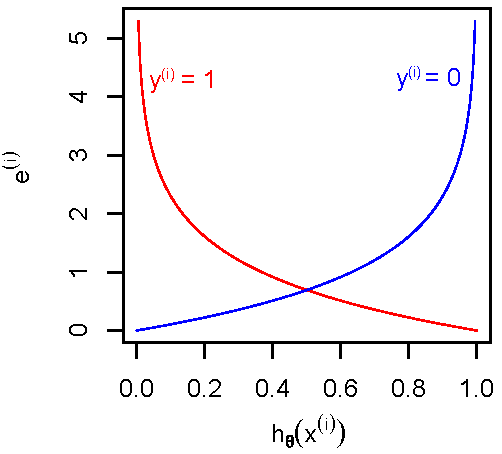
\includegraphics[width=0.5\columnwidth]{images/errori_logistica}
  \caption{Contributi all'errore nella regressione logistica}
  \label{fig:errori_logistica}
\end{figure}

\subsection{Metodo della discesa del gradiente}
Poiché non esiste un metodo analitico per minimizzare la funzione costo, l'unica l'alternativa è un metodo numerico, come quello basato sulla discesa del gradiente. Come già visto, questo metodo si basa sulla seguente regola di aggiornamento dei pesi:
\begin{equation*}
  \theta_k^{NEW} = \theta_k^{OLD} - \alpha \frac{ \partial J(\theta)}{ \partial \theta_k}.
\end{equation*}
Si vede facilmente che per la derivata della funzione logistica vale la seguente proprietà:
\begin{equation*}
g'(z) = \frac{\partial}{\partial z}\left( \frac{1}{1+e^{-z}}\right)=g(z)(1-g(z)).
\end{equation*}
Sfruttando la precedente nel calcolo delle derivate di $J(\theta)$ si vede che la regola di aggiornamento dei pesi è identica a quella della regressione lineare, cioè:
\begin{equation*}
   \theta_k^{NEW} = \theta_k^{OLD} - \alpha \frac{1}{m} \sum_{i=1}^m (h(x^{(i)})-y^{(i)}) x^{(i)}_k.\end{equation*}
Essa può essere applicata sia per il \emph{batch gradient descent} che per le sue varianti stocastiche.

\subsubsection{Derivazione della regola di aggiornamento dei pesi}\label{sec:dim_log_regr}
Vediamo ora quali sono i passaggi che portano all'espressione della regola di aggiornamento dei pesi\footnote{Approfondimento non trattato a lezione}. Come già detto, la derivata della funzione logistica gode della seguente proprietà:
\begin{equation*}
g'(z) =g(z)(1-g(z)).
\end{equation*}
Partendo da essa, calcoliamo la derivata parziale di $h_\theta(x)$, che tornerà utile in seguito:
\begin{equation*}
\frac{\partial h_\theta(x)}{\partial \theta_k} = h_\theta(x) (1-h_\theta(x)) \frac{\partial (\theta^T x)}{\partial \theta_k}
\end{equation*}
dove, come già visto in \autoref{sec:gradiente}, risulta che:
\begin{equation*}
\frac{\partial (\theta^T x)}{\partial \theta_k} = x_k
\end{equation*}
e quindi
\begin{equation*}
\frac{\partial h_\theta(x)}{\partial \theta_k} = h_\theta(x) (1-h_\theta(x)) x_k.
\end{equation*}
Passiamo ora al calcolo della derivata parziale di $J(\theta)$:

 \begin{equation}\label{eq:delta_j}
 \frac{\partial J(\theta)}{\partial \theta_k} = -\frac{1}{m}\sum_{i=1}^m \left( {y^{(i)}} \frac{\partial}{\partial \theta_k}(\log{h_\theta(x^{(i)})}) + (1-y^{(i)})
 \frac{\partial}{\partial \theta_k}(\log{(1 - h_\theta(x^{(i)}))}) \right).
\end{equation}
Esaminiamo separatamente le due derivate:
\begin{equation*}
\frac{\partial}{\partial \theta_k}\log{h_\theta(x^{(i)})} = \frac{1}{h_\theta(x^{(i)})} h_\theta(x^{(i)}) (1-h_\theta(x^{(i)})) x_k^{(i)} =  (1-h_\theta(x^{(i)})) x_k^{(i)}
\end{equation*}

\begin{equation*}
\frac{\partial}{\partial \theta_k}\log{(1 - h_\theta(x^{(i)}))} = \frac{1}{1- h_\theta(x^{(i)})} (-h_\theta(x^{(i)})) (1-h_\theta(x^{(i)})) x_k^{(i)} =  -h_\theta(x^{(i)}) x_k^{(i)}
\end{equation*}
Sostituiamo le precedenti nell'\autoref{eq:delta_j}, raccogliamo $x_k$ e sviluppiamo il prodotto per ottenere la derivata finale:

 \begin{dmath*}
 \frac{\partial J(\theta)}{\partial \theta_k} = -\frac{1}{m}\sum_{i=1}^m \left( {y^{(i)}} (1-h_\theta(x^{(i)})) x_k^{(i)} + (1-y^{(i)})
 (-h_\theta(x^{(i)})) x_k^{(i)} \right) 
 =-\frac{1}{m}\sum_{i=1}^m \left( {y^{(i)}} (1-h_\theta(x^{(i)})) + (1-y^{(i)})
 (-h_\theta(x^{(i)})) \right) x_k^{(i)}  
 = \frac{1}{m}\sum_{i=1}^m \left( h_\theta(x^{(i)}) - y^{(i)} \right) x_k^{(i)}  
\end{dmath*}

\subsection{Regressione logistica: caso multiclasse}
Con la regressione logistica siamo in grado di realizzare un classificatore binario. Se le classi sono più di due, si possono adottare due approcci:
\begin{enumerate}
\item usare una funzione logistica a più livelli (che non approfondiremo);
\item usare più funzioni logistiche in un approccio \emph{one-vs-all}, che ci apprestiamo ad approfondire.
\end{enumerate}
Supponiamo di dover distinguere $n$ classi, per farlo addestreremo $n$ classificatori (quindi avremo $n$ funzioni logistiche) ciascuno dei quali sarà in grado di identificare come classe 1 una classe desiderata, e tutte le altre $n-1$ saranno riconosciute come classe 0. Una volta addestrati gli $n$ classificatori, per classificare un nuovo ingresso lo diamo in \emph{input} a tutte le funzioni logistiche, ciascuna restituirà un valore tra 0 ed 1, quello più alto determinerà la classe di appartenenza dell'ingresso (cioè ci dirà quale classificatore ha dato la risposta più alta, presumibilmente quello specializzato sulla reale classe di appartenenza dell'ingresso). Di fatto in questo approccio interpretiamo l'uscita dell'\emph{i-esimo} classificatore come la probabilità che l'ingresso appartenga alla classe \emph{i-esima}.

\subsection{Regolarizzazione}
Uno dei problemi in cui è possibile incorrere è l'\emph{overfitting} e tramite la ``regolarizzazione'' possiamo evitarlo. 

L'idea di base è che, fissato il grado di un modello, il suo andamento sarà tanto più oscillatorio quanto più grandi saranno i $\theta_i$. La regolarizzazione, quindi, si propone di prevenire l'\emph{overfitting} penalizzando i $\theta_i$ grandi, senza agire direttamente sul grado del modello.

\subsubsection{Regolarizzazione con norma $\ell^2$}\label{sec:regolarizzazione_l2}

Il concetto di base è molto semplice: sommiamo alla funzione costo un qualcosa che penalizzi i $\theta_i$ grandi, nella fattispecie il nostro ``qualcosa'' è il quadrato della norma in modulo 2 del vettore 
 $\theta$ (escluso $\theta_0$ poiché è l'intercetta e non contribuisce all'andamento della funzione).

Nel caso della regressione lineare, la funzione costo regolarizzata prende il nome di \emph{Ridge Regression} ed è la seguente:
\begin{equation}\label{eqJ_theta}
  J(\theta) = \frac{1}{2m} \left(\sum_{i=1}^m (h(x^{(i)})-y^{(i)})^2 + \lambda \sum_{j=1}^n\theta_j^2\right)
\end{equation}
dove:
\begin{itemize}
\item $\sum_{j=1}^n\theta_j^2 = ||\theta||_2^2$; sommare questo contributo è equivalente a minimizzare $J(\theta)$ originale ponendo un vincolo sul valore massimo della norma;
\item $\lambda$ è detto parametro di regolarizzazione e determina l'influenza del fattore di regolarizzazione: più è grande, più piccoli saranno i $\theta$ e più smussata sarà l'ipotesi.
\end{itemize}
Nel caso della regressione logistica, questo approccio porta a riformulare la funzione costo come segue:
 \begin{equation*}
 J(\theta) = -\frac{1}{m}\sum_{i=1}^m \left( {y^{(i)}}\log{h_\theta(x^{(i)})} + (1-y^{(i)})
 \log{(1 - h_\theta(x^{(i)}))} \right) + \frac{\lambda}{2m}\sum_{j=1}^n\theta_j^2.
\end{equation*}
In maniera simile a quanto già fatto, possiamo calcolare le derivate delle funzioni costo regolarizzate e dedurre la regola di aggiornamento dei pesi. Si vede facilmente che, sia nel caso di regressione lineare che logistica, essa diventa:
\begin{gather*}\begin{cases}
\displaystyle\theta^{NEW}_0 = \theta^{OLD}_0 - \alpha \frac{1}{m} \sum_{i=1}^m \left(h_\theta(x^{(i)}) - y^{(i)}\right)x_0^{(i)} \\
\displaystyle\theta^{NEW}_k = \theta^{OLD}_k - \alpha \left[ \frac{1}{m} \sum_{i=1}^m \left(h_\theta(x^{(i)}) - y^{(i)}\right)x_k^{(i)}+\frac{\lambda}{m}\theta_k\right] \quad k=1,2,\dots,n
\end{cases}
\end{gather*}
La regola di aggiornamento di $\theta_0$ rimane invariata, come ci aspetteremmo sapendo che esso non è coinvolto nella regolarizzazione. Per tutti gli altri coefficienti possiamo riscrivere la regola come segue:
\begin{equation*}
\displaystyle\theta^{NEW}_k = \theta^{OLD}_k \left(1- \alpha\frac{\lambda}{m}\right) - \alpha \frac{1}{m} \sum_{i=1}^m \left(h_\theta(x^{(i)}) - y^{(i)}\right)x_k^{(i)} \quad k=1,2,\dots,n
\end{equation*}
Notiamo che la seconda parte della regola è identica alla versione senza regolarizzazione. In condizioni ``tipiche'' accade che $\alpha<1$, $\lambda > 0$ ed $m$ è piuttosto grande. Questo fa sì che il termine $\left(1- \alpha\frac{\lambda}{m}\right)$ sia minore di $1$. Ciò ci fornisce un'interessante interpretazione della nuova regola di aggiornamento. Infatti è come se l'algoritmo aggiornasse $\theta_k$ applicando la classica regola (senza regolarizzazione) a partire da una versione scalata del precedente valore di $\theta_k$ (poiché viene moltiplicato per una quantità minore di $1$).

\subsubsection{Regolarizzazione con norma $\ell^1$}
Un'ulteriore tecnica di regolarizzazione (detta \emph{lasso}) prevede di usare la norma $\ell^1$ piuttosto che il quadrato della norma $\ell^2$. 
Le espressioni precedenti rimangono invariate, ad eccezione dell'ultima sommatoria che viene sostituita da:
\begin{equation*}
\ell^1 = \sum_{j=1}^n|\theta_j|.
\end{equation*}
Questo tipo di sostituzione, però, implica che la nuova funzione costo $J(\theta)$ non sia più derivabile con continuità (a causa di $\ell^1$). 

Ma allora perché preferire $\ell^1$ ad $\ell^2$?

\subsubsection{$\ell^2$ vs $\ell^1$}
Le persone serie (non noi) hanno dimostrato le seguenti conclusioni.

\begin{figure}[]
\centering
  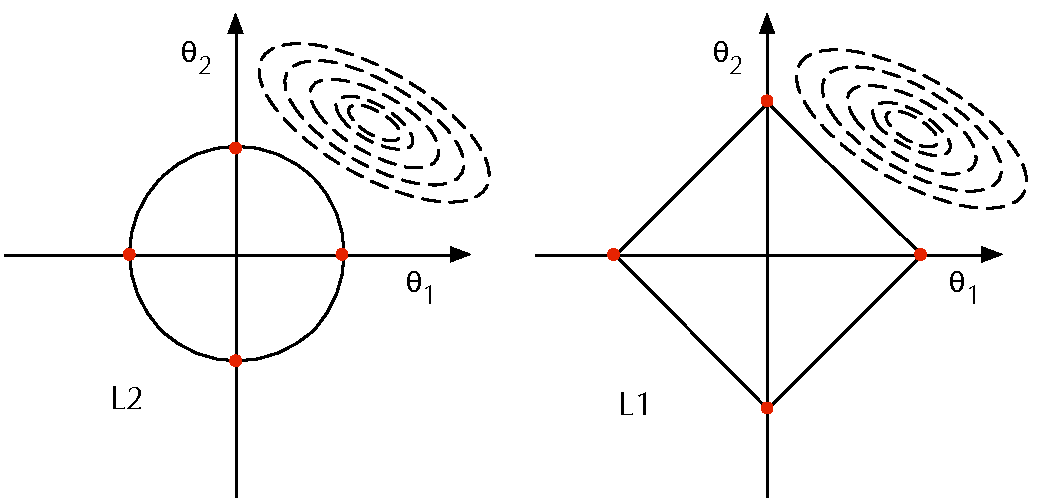
\includegraphics[width=\columnwidth]{images/norme}
  \caption{Regolarizzazione con norma $\ell^1$ ed $\ell^2$}
  \label{fig:norme}
\end{figure}

Come già detto, l'introduzione della norma nella funzione costo equivale ad imporre un limite al suo valor massimo. Possiamo quindi riscrivere i due problemi come segue (ignoriamo i fattori di normalizzazione $m$ al denominatore, senza che ciò cambi i risultati):

\begin{gather}
\text{Norma }\ell^2:
\quad \min\sum_{i=1}^m(\dots)^2 \\
\qquad \text{s.t.} \qquad ||\theta||_2^2 < t
\end{gather}
 
 \begin{gather}
\text{Norma }\ell^1:
\quad \min\sum_{i=1}^m(\dots)^2 \\
\qquad \text{s.t.} \qquad ||\theta||_1 < t
\end{gather}
Per capire i risultati ottenuti dalla gente seria, riconduciamoci al caso $n=2$, per cui le precedenti diventano:
\begin{gather}
\text{Norma }\ell^2:
\quad \min\sum_{i=1}^m(\dots)^2 \\
\qquad \text{s.t.} \qquad \theta_1^2 + \theta_2^2 < t
\end{gather}
 
 \begin{gather}
\text{Norma }\ell^1:
\quad \min\sum_{i=1}^m(\dots)^2 \\
\qquad \text{s.t.} \qquad |\theta_1|+|\theta_2| < t
\end{gather}
Sappiamo che:
\begin{itemize}
\item $\sum(\dots)^2$ rappresenta un paraboloide (tratteggiato in \autoref{fig:norme});
\item $\theta_1^2 + \theta_2^2 < t$ delimita l'area interna ad una circonferenza centrata nell'origine e di raggio $\sqrt{t}$ (vedi \autoref{fig:norme});
\item $|\theta_1|+|\theta_2| < t$ delimita l'area interna di un rombo di diagonale $2t$ (vedi \autoref{fig:norme}).
\end{itemize}
Lo scopo della minimizzazione è trovare $\theta_1$ e $\theta_2$ che minimizzano il paraboloide e ricadano nelle aree delimitate dal dominio. 



Si vede che, se questi punti ricadono nelle intersezioni tra il perimetro del dominio ed uno dei due assi, uno dei due $\theta_i$ sarà nullo (punti rossi in \autoref{fig:norme}). Se $\theta_i=0$ significa che l'attributo $x_i$ non comparirà nell'espressione del modello, ed avremo operato una \emph{feature selection} ``naturale''. Il motivo per cui la norma $\ell^1$ viene usata è perché si dimostra che comporta una maggiore probabilità di ricadere nelle intersezioni appena descritte, e quindi è molto utile per problemi con un gran numero di attributi (per contro occorre trovare un metodo alternativo alla discesa del gradiente che richiede la derivabilità della funzione costo).



\section{Progettazione di un sistema di ML}

La progettazione di un sitema di \emph{machine learning} può essere sintetizzata nelle seguenti fasi:
\begin{enumerate}
\item analisi e \emph{pre-processing} dei dati;
\item \emph{feature} selection;
\item scelta del modello ed addestramento;
\item validazione del modello sul \emph{validation set} ed eventualmente si ritorna al passo precedente;
\item valutazione delle prestazioni su un \emph{test set};
\item adozione del modello nel contesto finale.
\end{enumerate}
Analizziamo di seguito le singole fasi.

\subsection{Analisi e pre-processing dei dati}
\subsubsection{Pulizia dei dati}
I dati ricevuti e provenienti dal mondo reale potrebbero essere sporchi, ovvero:
\begin{itemize}
\item potrebbero essere incompleti, ad esempio alcuni valori di un attributo sono mancanti;
\item potrebbero essere inaccurati o discostarsi molto da quanto ci si aspetterebbe (ad esempio a causa di una digitazione errata da parte di un operatore umano).
\end{itemize}
Poiché vale la regola GIGO (Garbage In - Garbage Out) secondo cui un modello addestrato con dati sporchi produrrà risultati non affidabili, è necessario individuare tutte queste anomalie e ripulire i dati. Per quanto questa operazione non segua sempre un flusso standard, ma dipende dai particolari dati e dalle proprietà che possiamo osservare, si possono distinguere alcune operazioni comuni:
\begin{itemize}
\item rimozione degli \emph{outlier}: per \emph{outlier} si intendono gli esempi il cui valore d'uscita supera il terzo quartile (\autoref{sec:quantili});
\item rimozione dei duplicati: un campione d'addestramento duplicato non aggiunge alcune informazione utile;
\item rimozione del rumore: cioè delle informazioni inutili (ad esempio l'ID utente è tipicamente un valore non significativo ai fini della classificazione).
\end{itemize}

\paragraph{Quantili e quartili}\label{sec:quantili}
L'$\alpha$-quantile, con $\alpha \in [0,1]$, identifica quel valore $x_\alpha$ tale che una quota $\alpha$ della popolazione delle $x$ sia $\leq x_\alpha$.
Esistono diversi quantili tipicamente utilizzati, e sono:
\begin{itemize}
\item quartili, dividono la distribuzione in 4 parti uguali. Ciascun quartile rappresenta il 25\% della popolazione (quindi il terzo quartile è quel valore di $x$ di cui il 75\% della popolazione è più piccolo);
\item decili, dividono la popolazione in 10 parti uguali (ciascun decile rappresenta il 10\% della popolazione);
\item percentili, dividono la popolazione in 100 parti uguali (ciascuna parte rappresenta l'1\% della popolazione).
\end{itemize}

\subsubsection{Pre-processing}
Oltre ad aver pulito i dati è necessario pre-elaborarli prima di darli in pasto al classificatore, alcune operazioni comuni sono:
\begin{itemize}
\item discretizzazione ed aggregazione, ad esempio potremmo raggruppare gli ingressi in base all'attributo ``età'' in ``adulti'', ``ragazzi'' e ``bambini'';
\item normalizzazione e \emph{re-scaling} (trattate nel paragrafo successivo);
\item creazione di nuovi attributi, ad esempio quando adottiamo un GLM stiamo aumentando il numero di feature. Ciò è utile a patto che consenta una separazione più netta delle classi, se ciò non accade introduciamo una complicazione superfla al problema.
\end{itemize}

\paragraph{Normalizzazione e re-scaling}\label{feature_scaling}
La normalizzazione consiste nel restringere l'intervallo di variabilità di un attributo preservando le distanze relative tra i suoi valori. Il \emph{re-scaling} è un semplice cambio di scala, cioè divisione o moltiplicazione per uno stesso valore.

Queste operazioni si rendono necessarie perché ciascun attributo può variare in un intervallo più o meno ampio rispetto agli altri (ad esempio l'altezza ed il peso espressi in cm e kg hanno intervalli di variabilità molto diversi). Molti algoritmi di classificazione non riescono ad operare su dati così fatti, ad esempio la funzione logistica satura ad 1 quando l'ingresso è troppo grande. Anche lì dove questo problema non si presenta, come nella regressione lineare, si vede che l'algoritmo di discesa a gradiente converge più velocemente quando i dati sono normalizzati\footnote{\href{http://www.youtube.com/watch?v=PINX6Mk636M}{Coursera, Machine Learning (Andrew Ng), Lezione 4.3} }. Ribadiamo ulteriormente  che ciascun attributo viene normalizzato separatamente dagli altri e lo scopo della normalizzazione è far sì che tutti gli attributi varino in uno stesso intervallo. Una volta normalizzati gli ingressi, occorre memorizzare i parametri usati per la normalizzazione, in maniera tale che questa possa essere riapplicata invariata agli ingressi incontrati in fase di predizione. Le tecniche principali sono:
\begin{itemize}
\item \emph{min-max normalization}, si scalano i valori dell'attributo in funzione del minimo e del massimo per farli rientrare in un intervallo [a,b] desiderato (tipicamente [0,1]).
\begin{equation*}
x_i \leftarrow \frac{x_i - \min_i(x_i)}{\max_i(x_i) - \min_i(x_i)} \cdot (b-a) +a
\end{equation*}

\emph{Svantaggi:} 
\begin{enumerate}
\item gli \emph{outlier} influiscono molto su min e max, e quindi sulla normalizzazione;
\item in fase di predizione potrebbe arrivare un ingresso al di fuori dell'intervallo $[\min, \max]$ per cui la normalizzazione sarebbe errata (in risultato sarebbe più piccolo di $a$ o più grande di $b$).
\end{enumerate}
\item \emph{z-score normalization}, normalizza i valori nell'intervallo [-1,1] e si basa su valor medio e deviazione standard, quindi non subisce l'influenza degli \emph{outlier}.
\begin{equation*}
x_i \leftarrow \frac{x_i - \overline{x}}{\sigma_{x}}
\end{equation*}

\end{itemize}

\subsection{Feature selection}
Possono capitare spesso due scenari:
\begin{itemize}
\item nel \emph{dataset} sono presenti attributi superflui. Ad esempio in una base di dati che contiene $\langle$ID, altezza, peso, sesso$\rangle$, l'ID è superfluo ai fini della classificazione;
\item alcuni attributi sono linearmente dipendenti e quindi mantenerne uno solo è sufficiente, dato che tutti gli altri non aggiungi informazione. Ad esempio se il \emph{dataset} prevede $\langle$sesso, peso (kg), peso (lb)$\rangle$ è evidente che uno dei due pesi è eliminabile.
\end{itemize}

Ridurre le dimensioni dei vettori delle \emph{feature} consente di semplificare il problema e ciò si traduce in tempi di addestramento più brevi e modelli meno complessi (di grado inferiore, riducendo dunque il rischio di \emph{overfitting}).

Le tecniche adottate per individuare gli attributi superflui sono:
\begin{enumerate}
\item Filtri: grazie ai quali è possibile stabilire un \emph{ranking} degli attributi in cui gli ultimi sono quelli che discriminano meno la classe di appartenenza dell'esempio (misure tipiche: \emph{information gain}, \emph{entropy}, \emph{mutual information});
\item \emph{Wrappers:} si suddivide il \emph{set} di dati di addestramento in due parti. La prima parte viene utilizzata per addestrare il modello, selezionando però solo un sottoinsieme di attributi per volta. Per ciasucno di questi sottoinsiemi si valutano le prestazioni sulla seconda parte (\emph{validation set}) per capire quali attributi hanno influenza maggiore;
\item Algoritmi di riduzione della dimensionalità (PCA, trattata in seguito).
\end{enumerate}

\subsection{Scelta del modello}\label{sec:overunderfitting}
\subsubsection{Overfitting ed underfitting}
Nella scelta del modello è importante evitare due situazioni:
\begin{itemize}
\item \emph{overfitting}: si verifica quando il modello si comporta molto bene sul \emph{training set} ma non è in grado di prevedere correttamente le classi dei campioni nel \emph{validation set}. Significa che il modello non è in grado di generalizzare ed è quindi troppo complesso (grado troppo elevato). Un modello troppo complesso oscillerà molto e sarà caratterizzato da una forte varianza.
\item \emph{underfitting}: il modello è troppo semplice e genera errori troppo grandi sia sui dati di addestramento che su quelli di validazione. Ciò si traduce in un errore medio di predizione elevato (\emph{bias});
\end{itemize}

\subsubsection{Trade-off tra bias e varianza}
Cerchiamo di capire qual è l'influenza di \emph{bias} e varianza sull'errore mediamente commesso da un modello\footnote{Questa parte è stata scritta partendo dagli appunti ed integrandoli con il libro e con quanto letto \href{http://www-scf.usc.edu/~csci567/17-18-bias-variance.pdf}{qui}.}.

\paragraph{Formulazione del problema}
Ipotizziamo di avere a disposizione infiniti \emph{dataset} $D_i$ la cui unione costuituisce l'intera popolazione di campioni che il nostro modello potrà mai incontrare nella sua esistenza.

Ipotizziamo di fissare il tipo di modello da usare (ad esempio il grado del polinomio di una regressione lineare) e di addestrarlo ogni volta con un diverso $D_i$, otterremo quindi infinite ipotesi $h^{(D_i)}(x)$.

Ciascun campione del \emph{dataset} è nella forma $<\mathbf{x^{(i)}}, y^{(i)}>$ dove $y^{(i)}$ è somma di un valore vero (a noi sconosciuto) e di un errore gaussiano a media nulla e varianza $\sigma_e$:
\begin{equation*}
y^{(i)}=f(\mathbf{x^{(i)}})+e^{(i)}
\end{equation*}


Ciascuna delle ipotesi $h^{(D_i)}$ commetterà un errore nel predire i campioni \emph{rispetto al loro valore vero}, e lo possiamo esprimere sotto forma di errore quadratico medio (MSE):
\begin{equation*}
MSE\left(h^{(D_i)}(x)\right) =E_x\left[(h^{(D_i)}(x)-f(x))^2\right]
\end{equation*}

A noi interessa valutare l'aspettazione (valore atteso) di quest'ultima quantità rispetto ai $D_i$. In pratica è come se misurassimo l'errore quadratico  medio  commesso da ciascun singolo modello su tutti i possibili ingressi e mediassimo a loro volta questi risultati; ovviamente il calcolo di questo valor medio richiederebbe la conoscenza di tutti gli infiniti $D_i$, per cui ci accontentiamo del valore atteso (che chiameremo \emph{Generalization Error} o \emph{GER}):
\begin{dmath*}
GER = E_D[MSE] = E_D\left[E_x\left[\left(h^{(D_i)}(x)-f(x)\right)^2\right]\right] 
= E_x\left[E_D\left[\left(h^{(D)}(x^{(i)})-f(x^{(i)})\right)^2\right]\right]
\end{dmath*}

L'ultimo passaggio è possibile perché l'operatore $E$ è lineare (si tratta di una sommatoria nel caso discreto). Essendo tutti gli addendi di $E_x$ non negativi, per ottenere un \emph{GER} piccolo non ci resta che minimizzare $E_D$. La presenza degli apici  $(i)$ nella formula più interna, ci ricorda che l'aspettazione $E_D$ che desideriamo conoscere è calcolata fissato un singolo campione $x^{(i)}$ e facendo variare il modello usato.

\paragraph{Decomposizione}
Studiamo ora come è fatto il termine\footnote{La decomposizione del MSE in \emph{bias} e varianza è valida in generale. Qui riportiamo la dimostrazione usando la notazione del contesto in analisi.}:

\begin{equation}\label{eq-aspettazione}
E_D\left[\left(h^{(D)}(x^{(i)})-f(x^{(i)})\right)^2\right].
\end{equation}
Introduciamo la grandezza:
\begin{equation*}
\overline{h}(x^{(i)}) = E_D\left[h^{(D)}(x^{(i)})\right]
\end{equation*}
che rappresenta la media statistica dei valori restituiti in uscita da ciascun modello $h^{(D_i)}$ quando tutti ricevono in ingresso uno stesso $x^{(i)}$. In altre parole fissiamo $x^{(i)}$, lo diamo in pasto a tutti i modelli addestrati e calcoliamo la media delle uscite. Questa quantità rappresenterà la miglior stima di $f(x^{(i)})$.

A questo punto sommiamo e sottraiamo $\overline{h}(x^{(i)})$ nell'\autoref{eq-aspettazione}:

\begin{dmath*}
E_D\left[\left(h^{(D)}(x^{(i)})-\overline{h}(x^{(i)})+\overline{h}(x^{(i)})-f(x^{(i)})\right)^2\right]
\end{dmath*}
sviluppiamo il quadrato raggruppando gli addendi 2 per volta e sfruttiamo la linearità di $E$:
\begin{dmath*}
E_D\left[\left(h^{(D)}(x^{(i)})-\overline{h}(x^{(i)})\right)^2\right] +E_D\left[\left(\overline{h}(x^{(i)})-f(x^{(i)})\right)^2 \right]+ E_D\left[2\left( h^{(D)}(x^{(i)})-\overline{h}(x^{(i)})\right) \left( \overline{h}(x^{(i)})-f(x^{(i)})\right)\right]
\end{dmath*}
Analizziamo ora i singoli addendi. Il primo rappresenta, per definizione, la varianza:
\begin{equation*}
E_D\left[\left(h^{(D)}(x^{(i)})-\overline{h}(x^{(i)})\right)^2\right] = Var\left(h^{(D)}(x^{(i)})\right).
\end{equation*}
Nel secondo termine entrambi gli addendi non dipendono più da $D$, fissato un $x^{(i)}$ rappresentano dei numeri, per cui:
\begin{equation*}E_D\left[\left(\overline{h}(x^{(i)})-f(x^{(i)})\right)^2 \right]= (\overline{h}(x^{(i)})-f(x^{(i)}))^2
\end{equation*}
e questa quantità rappresenta per definizione il $Bias^2\left(h^{(D)}(x^{(i)})\right)$. Lo stesso discorso può essere fatto per il terzo fattore del terzo addendo:
\begin{dmath*}
2\left( \overline{h}(x^{(i)})-f(x^{(i)})\right)\left E_D[h^{(D)}(x^{(i)})-\overline{h}(x^{(i)}) \right] 
=2\left( \overline{h}(x^{(i)})-f(x^{(i)})\right) \left( E_D\left[ h^{(D)}(x^{(i)})\right]-E_D\left[\overline{h}(x^{(i)}) \right]\right)
=2\left( \overline{h}(x^{(i)})-f(x^{(i)})\right) \left(\overline{h}(x^{(i)})-\overline{h}(x^{(i)})\right)=0
\end{dmath*}

In definitiva:

\begin{dmath*}
MSE(h^{(D)}(x^{(i)})) 
= Bias^2\left(h^{(D)}(x^{(i)})\right) + Var\left(h^{(D)}(x^{(i)})\right).
\end{dmath*}

\paragraph{Commento dei risultati}
L'errore di generalizzazione di un modello è l'aspettazione del MSE appena definito, abbiamo quindi interesse a rendere l'MSE piccolo. Ciò può essere ottenuto riducendo il \emph{bias} o la varianza:
\begin{itemize}
\item il \emph{bias} tiene conto di quanto la migliore stima (cioè la media delle stime) sia in grado di avvicinarsi al valore vero. Un \emph{bias} alto è indice di un modello troppo semplice che, a prescindere dal \emph{dataset} $D_i$ di addestramento, non ha una buona capacità predittiva. Questo è riconducibile ad un polinomio di grado troppo basso;
\item la varianza tiene conto di quanto ciascuna ipotesi si discosta dal valor medio calcolato su tutte le ipotesi. Una varianza alta è indice del fatto che, addestrando uno stesso modello con $D_i$ diversi, si possono ottenere ipotesi molto diverse. Ciò significa che il modello è troppo complesso, tende ad andare in \emph{overfitting} e manca di capacità di generalizzazione.
\end{itemize}


L'ideale sarebbe avere sia \emph{bias} che varianza piccoli, ciò garantisce che il modello approssimi bene i risultati reali pur rimanendo stabile, cioè non subisce fortemente l'influenza del particolare \emph{training set} utilizzato (a patto che questo sia ben costruito). In \autoref{fig:bias_vs_varianza} è mostrato il tipico andamento di \emph{bias} e varianza in funzione della complessità del modello. Notiamo che le due componenti hanno un andamento opposto (al diminuire dell'una, aumenta l'altra), il miglior compromesso è rappresentato dal punto in cui la loro somma è minima.

\begin{figure}[tbp]
\centering
  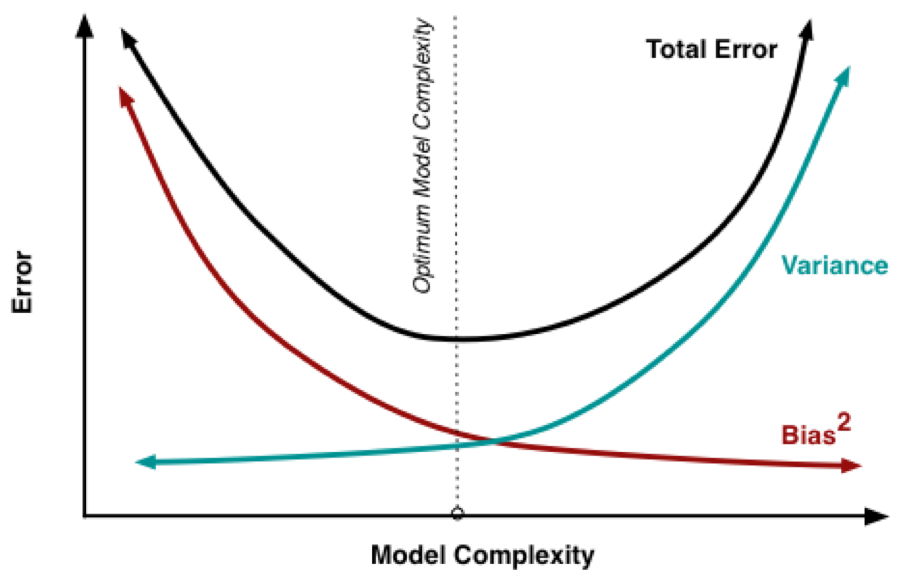
\includegraphics[width=0.6\textwidth]{images/bias_vs_var}
  \caption{\emph{Bias} e varianza in funzione della complessità del modello.}
  \label{fig:bias_vs_varianza}
\end{figure}


\subsubsection{Cross-validation}

Non sapendo quale modello scegliere, l'idea della \emph{cross-validation} è quella di addestrarne alcuni su un sottoinsieme del \emph{training set} a disposizione e poi valutarne le prestazioni sulla restante parte (\emph{validation set}).

La scelta del modello finale va fatta sulla base delle misure di prestazione calcolate sul \emph{validation set} e non sul \emph{training set}. Questo ha senso perché il modello è stato addestrato per minimizzare l'errore quadratico sul \emph{training set} ed in virtù di  ciò ci aspettiamo che l'errore commesso su di esso sia basso. In particolare, si dimostra che l'errore commesso su \emph{training set} è una sottostima dell'errore di generalizzazione, mentre quello sul \emph{validation set} lo approssima in maniera migliore.

Dopo aver scelto quale modello usare, questo può essere riaddestrato utilizzando tutto il \emph{training set} iniziale.

Questo stesso approccio può essere sfruttato per determinare metaparametri (ad esempio il coefficiente di penalizzazione del fattore di regolarizzazione) oppure per capire quali siano le \emph{feature} meno significative.

Due tecniche comunemente usate per effettuare \emph{cross-validation} prendono il nome di \emph{holdout} e \emph{k-folds}

\begin{figure}[]
\centering
  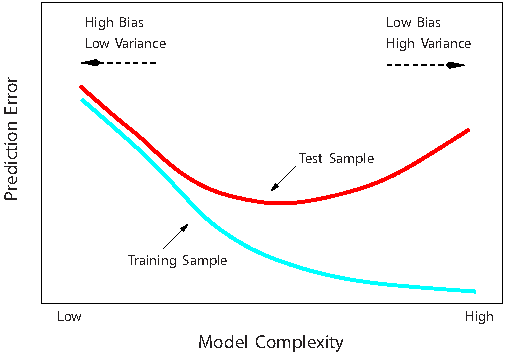
\includegraphics{images/bias_varianza}
  \caption{Errore di predizione su \emph{trainig set} e \emph{validation set} al variare della complessità del modello}
  \label{fig:bias_varianza}
\end{figure}

\subsubsection{Holdout cross validation}
La \emph{holdout cross validation} prevede che il \emph{training set } su cui addestrare i modelli in prova sia costituito dai due terzi di quello iniziale, il restante terzo costituirà il \emph{validation set}. Occorre prestare attenzione affinché i campioni scelti per l'addestramento e per la valutazione siano rappresentativi di tutte le classi presenti. Se ad esempio la classe 0 è completamente assente tra i dati di addestramento, e presente in quelli di validazione, il modello mostrerà una pessima capacità di riconoscere tali campioni e ciò si ripercuoterà negativamente sulle misure di prestazione.


\subsubsection{K-folds cross validation}
Questa tecnica prevede che l'insieme dei dati venga suddiviso in $k$ sottoinsiemi (tipicamente $k=10$). Durante ciascuna delle $k$ iterazioni dell'algoritmo, ciascun modello viene addestrato sull'unione di $k-1$ sottoinsiemi, e validato sul $k-esimo$. Ad ogni iterazione si cambiano i $k-1$ sottoinsiemi di addestramento e di conseguenza il $k-esimo$. L'errore commesso da ciascun modello viene calcolato come media degli errori da esso commessi in seguito a ciascuno dei $k$ addestramenti.

\subsection{Valutazione del modello}
La valutazione finale del modello viene fatta dopo averlo scelto, e quindi dopo averlo riaddestrato usando l'unione di \emph{training set} e \emph{validation set}. È evidente, quindi, che il \emph{test set} su cui valutiamo le prestazioni del modello debba essere distinto dagli altri due.

Occorre, inoltre, evitare il \emph{peeking}, cioè non usare i dati del \emph{test set} come se fossero parte del \emph{validation set}. In questa maniera il \emph{test set} viene usato per guidare la scelta del modello (è grave quasi come usare il \emph{test set} per l'addestramento), mentre per ottenere misure di prestazione credibili il \emph{test set} non deve avere alcuna influenza su come il modello viene scelto ed addestrato.


\subsubsection{Matrice di confusione e metriche}
La matrice di confusione consente di rappresentare in maniera compatta alcune grandezze di interesse per il calcolo delle misure di prestazione di un classificatore binario. Supponendo che l'uscita del classificatore sia \emph{yes} ($y=1$) o \emph{no} ($y=0$), la matrice di confusione viene costruita indicando sulle righe la classe reale dei campioni del \emph{test set}, sulle colonne la classe predetta dal classificatore per tali campioni (\autoref{fig:confusione}).



All'interno della matrice indichiamo 4 quantità:
\begin{itemize}
\item TP (\emph{true positive}), rappresenta il numero di veri positivi, cioè il numero di campioni classificati come positivi (classe 1) e che effettivamente sono positivi;
\item TN (\emph{true negative}), rappresenta il numero di veri negativi, cioè il numero di campioni classificati come negativi (classe 0) e che effettivamente sono negativi;
\item FP (\emph{false positive}), rappresenta il numero di falsi positivi, cioè il numero di campioni classificati come positivi (classe 1), ma che in realtà sono negativi;
\item FN (\emph{false negative}), rappresenta il numero di falsi negativi, cioè il numero di campioni classificati come negativi (classe 0), ma che in realtà sono positivi.
\end{itemize}
Osserviamo che:
\begin{itemize}
\item TP+TN+FP+FN è il  numero totale di campioni nel \emph{test set};
\item TP+FN è il numero di istanze positive nel \emph{test set};
\item TN+FP è il numero di istanze negative nel \emph{test set};
\item TP+FP è il numero di predizioni positive a partire dal \emph{test set};
\item TN+FN è il numero di predizioni negative a partire dal \emph{test set}.
\end{itemize}
Partendo da queste 4 quantità si definiscono alcune metriche di uso comune:
\begin{itemize}
\item \emph{Accuracy}, rappresenta il tasso di predizioni corrette:
\begin{equation*}
Accuracy = \frac{TP + TN}{TP+TN+FP+FN}
\end{equation*}
\item \emph{Error rate}, rappresenta il tassso di predizioni errate (complemento ad 1 dell'\emph{accuracy}):
\begin{equation*}
Error~Rate = 1 - Accuracy = \frac{FP + FN}{TP+TN+FP+FN}
\end{equation*}
\end{itemize}

\begin{figure}[]
\centering
  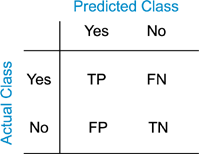
\includegraphics[width=0.3 \textwidth]{images/confusionmatrix}
  \caption{Matrice di confusione}
  \label{fig:confusione}
\end{figure}


Le due metriche precedenti tengono conto delle prestazioni complessive del classificatore. Non ci consentono di capire quanto sia buono nel discriminare casi positivi e casi negativi. A tal proposito vengono adottate le seguenti misure:
\begin{itemize}
\item \emph{Recall}, detta anche \emph{Sensitivity} o \emph{True Positive Rate}, rappresenta la percentuale di casi positivi correttamente calssificati:
\begin{equation*}
Recall = \frac{TP}{TP+FN}
\end{equation*}
\item \emph{Specificity}, detta anche  \emph{True Negative Rate}, in maniera duale alla precedente rappresenta la percentuale di casi negativi correttamente calssificati:
\begin{equation*}
Specificity = \frac{TN}{TN+FP}
\end{equation*}
\item \emph{False Positive Rate}, rappresenta il complemento ad uno della \emph{Specificity}, cioè la percentuale di casi negativi erroneamente classificati:
\begin{equation*}
False~Positive~Rate = 1 - Specificity =  \frac{FP}{TN+FP}
\end{equation*}
\end{itemize}
In ultimo può essere interessante valutare la \emph{Precision}, cioè il tasso di predizioni vere che si rivelano corrette, ovvero il rapporto tra i veri positivi e tutti i positivi:
\begin{equation*}
Precision = \frac{TP}{TP+FP}.
\end{equation*}
Tipicamente vorremmo un classificatore con \emph{Recall} e \emph{Precision} alte, cioè un classificatore con un alto numero di veri positivi e pochi falsi negativi e falsi positivi. Per unire queste due esigenze in un'unica metrica viene introdotta la \emph{F-measure}, calcolata come media armonica di \emph{Precision} e \emph{Recall}:
\begin{equation*}
\text{\emph{F-measure}} = 2\frac{Precision \cdot Recall}{Precision+Recall}.
\end{equation*}


\subsubsection{Curve ROC}

\begin{figure}[tbp]
\centering
  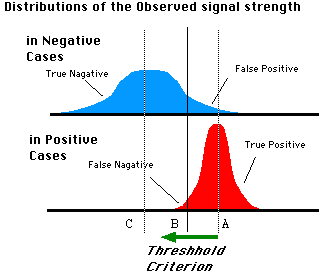
\includegraphics[width=0.5 \textwidth]{images/ROC_distribuzione}
  \caption{Distribuzione delle uscite associate ai campioni positivi e negativi nel \emph{test set}}
  \label{fig:ROC_distribuzione}
\end{figure} 
Vediamo ora come è possibile usare le informazioni provenienti dalle metriche appena introdotte per effettuare il \emph{tuning} di alcuni parametri del modello. 

Ipotizziamo di lavorare con una regressione logistica. Come abbiamo visto in precedenza, l'uscita della funzione ipotesi è numerica ed è compresa tra 0 ed 1. La classe di appartenenza di ciascun campione viene calcolata in base al fatto che tale uscita superi o meno un valore di soglia (\emph{threshold}). In precedenza, però, non abbiamo discusso su come debba essere scelta questa soglia.

Supponiamo che le distribuzioni delle uscite che il classificatore associa ai campioni di classe $1$ e $0$ del \emph{test set} siano gaussiane, rappresentate rispettivamente in azzurro e rosso in \autoref{fig:ROC_distribuzione}.


Se B rappresenta il valore di soglia scelto, è facile vedere che:
\begin{itemize}
\item i campioni negativi a sinistra di B rappresentano i veri negativi;
\item i campioni negativi a destra di B rappresentano i falsi positivi;
\item i campioni positivi a sinistra di B rappresentano i falsi negativi;
\item i campioni positivi a destra di B rappresentano i veri positivi.
\end{itemize}
Quindi la scelta della soglia influisce direttamente sulla matrice di confusione, e quindi sulle metriche analizzate. 

Tramite le curve ROC siamo in grado di vedere esattamente come il valore della soglia influisce sul \emph{True Positive Rate} e sul \emph{False Positive Rate}. Per tracciare una curva ROC facciamo variare la soglia in un intervallo di possibili valori, per ciascun valore calcoliamo \emph{True Positive Rate} e \emph{False Positive Rate} e disegniamo il punto individuato da questa coppia di valori su un sistema di assi cartesiani. La curva risultante rappresenterà l'andamento di \emph{TPR} e \emph{FPR} al variare della soglia (\autoref{fig:ROC}). A seconda di quali sono le esigenze del caso specifico, sceglieremo il valore di soglia più opportuno.

\begin{figure}[tbp]
\centering
  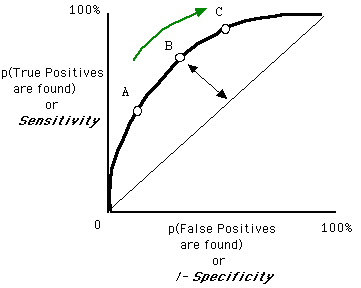
\includegraphics[width=0.5 \textwidth]{images/ROC}
  \caption{Curva ROC}
  \label{fig:ROC}
\end{figure}

Ad esempio, ipotizziamo che il sistema che stiamo addestrando consenta di classificare un paziente come sano o malato. Ovviamente vorremmo che esso fosse in grado di rivelare il 100\% dei malati, ovvero ottenere un \emph{TPR} pari ad 1. Paradossalmente potremmo ottenere ciò impostando una soglia nulla in maniera tale che tutti i pazienti vengano riconosciuti come malati, a prescindere dall'effettivo stato di salute. Da un punto di vista medico questo implicherebbe ulteriori esami sui pazienti per verificare l'effettiva presenza della malattia, e quindi un costo superiore da sostenere (per il paziente o per la Sanità Pubblica). Quindi ciò che vorremmo fare è anche minimizzare il \emph{FPR}, ed ecco che la curva ROC ci consente di individuare il giusto compromesso tra un \emph{TPR} alto ed \emph{FPR} basso. 
Nello stesso scenario, però, potremmo ipotizzare che la malattia sia grave e quindi potrebbe essere preferibile qualche falso positivo in più pur di non abbassare il tasso di veri positivi, evitando quindi che alcuni pazienti malati non vengano riconosciuti come tali. Anche in questo caso l'analisi della curva ROC può farci capire quale sia il miglior valore della soglia.

Le curve ROC possono essere usate anche per determinare i valori ottimali di altri metaparametri del modello, o per fare un confronto tra modelli diversi. In particolare possiamo tracciare la curva ROC di uno stesso modello, addestrato sullo stesso \emph{training set}, modificando di volta in volta il valore un metaparametro. Dopo ciascun addestramento possiamo tracciare la curva ROC e selezionare il modello la cui curva è migliore, cioè quella che sottende l'area maggiore, avvicinandosi maggiormente all'andamento ideale costante di una una retta passante per \emph{TPR}=1. 
\section{Algoritmi di classificazione non lineari}
\subsection{Reti neurali artificiali}
Vedi AIMA, Volume 2, paragrafo 20.5.

\subsection{Support Vector Machine}
Lo scopo di questi modelli è la classificazione binaria. Analizzeremo inizialmente il caso in cui i dati da classificare siano linearmente separabili, in seguito estenderemo il discorso a dati non linearmente separabili\footnote{Qualcosa su questo argomento si trova in AIMA, Volume 2, paragrafo 20.6. Per gli amanti del brivido, \href{http://www.disp.uniroma2.it/users/piccialli/svm_sciandrone.pdf}{questa} dispensa sembra decisamente più completa.}.

\subsubsection{Dati linearmente separabili}
Il modello che costruiamo è ancora una volta un iperpiano (come la regressione lineare ed il \emph{perceptron}), ma cambierà il modo in cui lo addestreremo, ovvero cambierà lo scopo dell'addestramento. L'espressione dell'ipotesi è quindi:
\begin{equation*}
h(\mathbf{x}) = \mathbf{w}^T \mathbf{x} + b.
\end{equation*}
Porre $h(\mathbf{x})=0$ ci consente di definire l'equazione dell'iperpiano separatore:
\begin{equation*}
\mathbf{w}^T \mathbf{x} + b = 0.
\end{equation*}
A questo punto, tutti i punti che si trovano al di sopra dell'iperpiano verrano classificati come $y=+1$, quelli al di sotto del piano come $y=-1$. Fare ciò è equivalente a porre l'uscita della funzione ipotesi in ingresso alla funzione segno, ovvero:
\begin{equation*}
y(\mathbf{x}^{(i)}) = \sign(h(\mathbf{x}^{(i)})) = \sign(\mathbf{w}^T \mathbf{x}^{(i)} + b).
\end{equation*}
Possiamo esplicitare l'espressione precedente come segue:
\begin{gather*}
\mathbf{w}^T \mathbf{x}^{(i)} + b > 0 \quad \rightarrow \quad y^{(i)} = +1 \\
\mathbf{w}^T \mathbf{x}^{(i)} + b < 0 \quad \rightarrow \quad y^{(i)} = -1 
\end{gather*}

A questo punto vediamo come determinare il vettore dei parametri $\mathbf{w}$ e $b$, cioè come determinare l'iperpiano separatore. Lo scopo della procedura di ottimizzazione che vogliamo costruire è massimizzare il \emph{margine}. Il margine si ottiene sommando un contributo $d^+$ ed un contributo $d^-$. $d^+$ rappresenta la minima distanza tra un punto di classe $+1$ e l'iperpiano separatore. $d^-$ è il corrispettivo per la classe $-1$, cioè la distanza minore tra un punto di classe $-1$ e l'iperpiano. I punti che danno origine a tale distanza, cioè i più vicini all'iperpiano, costituiscono i due \emph{vettori di supporto}.

Prima di formalizzare il problema di ottimizzazione, imponiamo due vincoli che ci torneranno utili in seguito: per tutti i punti appartenenti ai vettori di supporto l'ipotesi deve valere esattamente $+1$ o $-1$ (a seconda che il punto appartenga al vettore di supporto positivo o negativo):
\begin{gather*}
\mathbf{w}^T \mathbf{x}^{(i)} + b = +1 \quad \text{se }  \mathbf{x}^{(i)} \in s.v.^+\\
\mathbf{w}^T \mathbf{x}^{(i)} + b = -1 \quad \text{se }  \mathbf{x}^{(i)} \in s.v.^-
\end{gather*}

A questo punto possiamo sintetizzare i 4 vincoli imposti nell'unica espressione:
\begin{equation*}
y^{(i)}\left(\mathbf{w}^T \mathbf{x}^{(i)} + b\right) -1 \geq 0
\end{equation*}
vediamo perché questa ha senso:
\begin{itemize}
\item se  $\mathbf{x}^{(i)}$ è di classe $+1$, risulta $y^{(i)}=+1$ e quindi il vincolo precedente impone che $\mathbf{w}^T \mathbf{x}^{(i)} + b \geq +1$;
\item se  $\mathbf{x}^{(i)}$ è di classe $-1$, risulta $y^{(i)}=-1$ e quindi il vincolo precedente impone che $\mathbf{w}^T \mathbf{x}^{(i)} + b \leq -1$.
\end{itemize}
Torniamo al problema di massimizzazione: è noto\footnote{\href{http://mathworld.wolfram.com/Point-PlaneDistance.html}{Point-Plane Distance}}  che la distanza tra un generico $\mathbf{x}^{(i)}$ ed un iperpiano è pari a\footnote{Nelle slide del corso il numeratore è $|(\mathbf{w}^T \mathbf{x}^{(i)} + b) \cdot  y^{(i)}|$. Probabilmente questo è errato e l'introduzione di $y^{(i)}$ serve ad eliminare il valore assoluto. Infatti, per come abbiamo impostato il problema, risulta che $|(\mathbf{w}^T \mathbf{x}^{(i)} + b)| = (\mathbf{w}^T \mathbf{x}^{(i)} + b) \cdot  y^{(i)}$ (cioè $|x| = x \cdot \sign(x)$).}:
\begin{equation*}
\frac{ |(\mathbf{w}^T \mathbf{x}^{(i)} + b)|} {||\mathbf{w}||}
\end{equation*}
dove ricordiamo che:
\begin{itemize}
\item $||\mathbf{w}|| = \sqrt{\sum_{i=0}^n{w_i^2}}$
\end{itemize}
In base alle condizioni imposte, i punti dei vettori di supporto rendono unitario il numeratore della precedente, per cui il margine ($d^+ + d^-$) è proprio $\frac{2}{||\mathbf{w}||}$.

Il problema desiderato è quindi il seguente: vogliamo trovare $\mathbf{w}$ e $b$ che massimizzino $\frac{2}{||\mathbf{w}||}$ sotto i seguenti vincoli:
\begin{equation*}
y^{(i)}\left(\mathbf{w}^T \mathbf{x}^{(i)} + b\right) -1 \geq 0 \qquad i=1, \dots, m.
\end{equation*}
Si vede che:
\begin{equation*}
\argmax_{\mathbf{w},b}{\frac{2}{||\mathbf{w}||}} = \argmin_{\mathbf{w},b}{\frac{||\mathbf{w}||^2}{2}}.
\end{equation*}
Ciò ci consente di passare da una massimizzazione ad un problema di minimizzazione convesso e con vincoli di disuguaglianza lineari. In realtà a partire da quest'ultima formulazione (detta \emph{primale}) si genera il problema \emph{duale} (facendo utilizzo della funzione di Lagrange) che è di più semplice risoluzione. La funzione obiettivo diventa quindi:
\begin{equation*}
L(\mathbf{w}, b, \boldsymbol\alpha) = \frac{1}{2} ||\mathbf{w}||^2 - \sum_{i=1}^m \alpha_i ( y^{(i)} (\mathbf{w}^T \mathbf{x}^{(i)} + b)-1 ).
\end{equation*}


 Tramite una serie di passaggi ed osservazioni è possibile riformulare il problema come segue\footnote{C'è una differenza tra il libro e le slide, qui ho riportato la versione del libro di pag. 440 del secondo volume (paragrafo 20.6).
 
 Inoltre credo che per $\mathbf{x^{(i)}}\cdot\mathbf{ x^{(j)}}$ gli autori intendano il prodotto scalare tra due vettori di ingressi. Se così fosse, per correttezza formale,  il primo dovrebbe essere trasposto.}:
\begin{gather*}
\max_{\boldsymbol\alpha} \sum_{i=1}^m \alpha_i - \frac{1}{2} \sum_{i,j=1}^m y^{(i)} y^{(j)} \alpha_i \alpha_j (\mathbf{x^{(i)}}\cdot\mathbf{ x^{(j)}} )\\
s.t. \qquad \alpha_i \geq 0 \quad i=1,\dots,m \\
\sum_{i=1}^m \alpha_i y^{(i)} = 0
\end{gather*}
dove $\alpha_i$ sono i coefficienti di Lagrange introdotti dall'omonima funzione ed a partire dai loro valori ottimi è possibile ricavare $\mathbf{w}^*$ e $b^*$. Si vede che $\alpha_i$ è non nullo per tutti e soli i punti appartenenti ai vettori di supporto.

Una volta individuati il vettore di coefficienti ottimi $\boldsymbol\alpha^*$ è possibile passare alla soluzione del problema primario tramite due relazioni:
\begin{itemize} 
\item la prima consente di trovare i coefficienti ottimi dell'iperpiano ($\mathbf{w}^*$)
\begin{equation}\label{eq:w_ottimo}
w^* = \sum_{i=1}^m \alpha_i^* y^{(i)} x^{(i)};
\end{equation}
\item il secondo \emph{set} di equazioni consente di trovare il valore ottimo dell'intercetta ($b^*$)
\begin{equation*}
\alpha_i^* -  ( y^{(i)} (\mathbf{w}^{*T} \mathbf{x}^{(i)} + b^*)-1 )=0 \quad i=1,\dots,m
\end{equation*}
\end{itemize}
In particolare, soluzione trovata gode di alcune proprietà:
\begin{itemize}
\item $\alpha_i^*=0$ per tutti i punti che non giacciono sui margini;
\item $\alpha_i^*\neq0$ per tutti i punti che giacciono sui margini, cioè per quei punti facenti parte dei vettori di supporto.
\end{itemize}
Date le due precedenti conclusioni e l'\autoref{eq:w_ottimo}, notiamo che \emph{la soluzione ottima è una combinazione lineare dei soli vettori di supporto}. Quindi, l'equazione del piano separatore ottimo è:
\begin{equation*}
\mathbf{w}^{*T} \mathbf{x} + b^* = \sum_{i \in \{s.v.^+~\cup~s.v.^-\}} \alpha_i^* y^{(i)}(\mathbf{x}^{(i)T} \cdot \mathbf{x}) + b^*
\end{equation*}

\subsubsection{Soft margin SVM}
Esaminiamo ora come usare una SVM nel caso in cui i dati \emph{non} siano linearmente separabili. Notiamo che nella formulazione originale del problema ciascun vincolo
\begin{equation*}
y^{(i)}\left(\mathbf{w}^T \mathbf{x}^{(i)} + b\right) -1 \geq 0 \qquad i=1, \dots, m
\end{equation*}
impone che il punto \emph{i-esimo} non oltrepassi il semispazio delimitato dall'iperpiano in cui risiedono tutti i campioni della sua stessa classe. In altre parole, se un generico $\mathbf{x}^{(i)}$ è di classe $y$ il problema di ottimizzazione ammette soluzione solo se esiste una soluzione in cui tutti i punti si trovano nel semipiano ``corretto''. In caso di \emph{outlier} questa procedura non può funzionare. Ecco dunque che per contemplare la possibilità di ``far commettere errori'' alla procedura di ottimizzazione introduciamo per ciascun vincolo una variabile \emph{slack} $\xi_i \geq 0$. Il valore di ogni $\xi_i$ è proporzionale a quanto $\mathbf{x}^{(i)}$ sta ``sforando'' nel semipiano errato, cioè a quanto il punto anomalo si discosta dall'iperpiano e se è maggiore di $1$ indica una misclassificazione. I vincoli diventano quindi:
\begin{equation*}
y^{(i)}\left(\mathbf{w}^T \mathbf{x}^{(i)} + b\right) -1 + \xi_i \geq 0 \qquad i=1, \dots, m.
\end{equation*}
Ovviamente è necessario penalizzare i punti misclassificati, introducendo un fattore additivo nella funzione costo:
\begin{equation*}
\min_w \frac{1}{2} ||\mathbf{w}||^2 + C \sum_{i=1}^m \xi_i
\end{equation*}
dove $C$ rappresenta un parametro di \emph{regolarizzazione} il cui valore può essere determinato tramite \emph{cross validation}. Infatti una $C$ troppo grande rischia di produrre un addestramento troppo ``severo'' e non trovare una soluzione, il contrario produce un addestramento troppo tollerante e dunque un modello che genera troppi errori di classificazione. Il problema duale, quello effettivamente risolto, diventa:
\begin{gather*}
\max_\alpha \sum_{i=1}^m \alpha_i - \frac{1}{2} \sum_{i,j=1}^m y^{(i)} y^{(j)} \alpha_i \alpha_j (\mathbf{x^{(i)}}\cdot\mathbf{ x^{(j)}} )\\
s.t. \qquad 0 \leq \alpha_i \leq C \quad i=1,\dots,m \\
\sum_{i=1}^m \alpha_i y^{(i)} = 0.
\end{gather*}

\subsubsection{Metodi kernel}
Quanto appena visto non risolve tutti i problemi, infatti affinché il metodo funzioni è necessario che i punti siano distributi in regioni di spazio ``quasi'' linearmente separabili, cioè ammettiamo la presenza di \emph{outlier} ma non di non-linearità. L'idea alla base dei metodi \emph{kernel} è simile a quella delle funzioni di base ($\phi$), le quali applicano una funzione a ciascuna istanza di ingresso che ne aumenta il numero di \emph{feature} e renda linearmente separabili i campioni in uno spazio degli \emph{input} a dimensionalità superiore. 

Il problema in tutto ciò sorge quando le non-linearità sono molto forti e quando i vettori delle \emph{feature} sono molto grandi già prima dell'applicazione delle funzioni di base. Nell'espressione da ottimizzare compare infatti il prodotto $\mathbf{x}^{(i)} \mathbf{x}^{(j)}$:
\begin{equation*}
\max_\alpha \sum_{i=1}^m \alpha_i - \frac{1}{2} \sum_{i,j=1}^m y^{(i)} y^{(j)} \alpha_i \alpha_j (\mathbf{x}^{(i)} \mathbf{x}^{(j)}).
\end{equation*}
Dopo aver applicato le funzioni base, questo prodotto viene sostituito da $\phi(\mathbf{x}^{(i)})^T\phi(\mathbf{x}^{(j)})$ e questo calcolo può diventare oneroso nelle condizioni sopra descritte. Lo scopo di una funzione kernel $k(\mathbf{x}^{(i)}, \mathbf{x}^{(j)})$\footnote{Vedi le slide per alcuni esempi di funzioni kernel. 

Per rappresentare gli ingressi sto continuando ad usare la notazione introdotta fin dall'inizio, pur essendo leggermente diversa da quella delle slide e del libro.} è quello di restituire lo stesso risultato del precedente prodotto tra vettori, senza però richiedere una trasformazione esplicita degli ingressi, cioè:
\begin{equation*}
k(\mathbf{x}^{(i)}, \mathbf{x}^{(j)}) = \phi(\mathbf{x}^{(i)})^T\phi(\mathbf{x}^{(j)}).
\end{equation*}
Applicando una funzione simile, il problema di ottimizzazione diventa:
\begin{gather*}
\max_\alpha \sum_{i=1}^m \alpha_i - \frac{1}{2} \sum_{i,j=1}^m y^{(i)} y^{(j)} \alpha_i \alpha_j k(\mathbf{x}^{(i)},\mathbf{x}^{(j)}). \\
s.t. \qquad 0 \leq \alpha_i \leq C \quad i=1,\dots,m \\
\sum_{i=1}^m \alpha_i y^{(i)}= 0.
\end{gather*}
A questo punto la procedura di ottimizzazione richiede la scelta di:
\begin{itemize}
\item tipo di Kernel da usare;
\item parametri del Kernel scelto;
\item valore di C;
\end{itemize}
questi possono essere tutti determinati euristicamente tramite \emph{cross-validation}. Il vantaggio di pochi parametri da calibrare si aggiunge ai vantaggi delle SVM, cioè:
\begin{itemize}
\item la funzione da minimizzare è quadratica, e non c'è il pericolo di incappare in minimi locali;
\item la soluzione  può essere trovata in tempo polinomiale tramite le note tecniche di ottimizzazione;
\item le soluzioni sono stabili, cioè non dipendono da inizializzazioni casuali, come nel caso delle reti neurali;
\item la soluzione è sparsa, in quanto dipende solo dai vettori di supporto.
\end{itemize}

\subsection{K-nearest neighbors}
Vedi AIMA, Volume 2, paragrafo 20.4.

\section{Apprendimento statistico}
In questa parte analizzeremo un esempio di classificatore basato su apprendimento statistico: il classificatore \emph{bayesiano naive}. Esso  consente di predirre la classe di appartenenza di un campione sfruttando le regole della statistica, in particolar modo il suo funzionamento è incentrato sulla regola di \emph{Bayes}\footnote{AIMA, Volume 2, paragrafi 20.1 e 20.2 (il capitolo 13 è propedeutico).}.

\subsection{Regola di Bayes}
Dati due eventi $A$ e $B$, la regola di Bayes ci consente di calcolare la cosidetta ``probabilità a posteriori'', cioè la probabilità che dato l'evento $B$ si verifichi anche $A$. Essa è:
\begin{equation*}
p(A|B) = \frac{p(A,B)}{P(B)}.
\end{equation*}
Per la regola del prodotto possiamo scrivere:
\begin{equation*}
p(A,B) = p(A|B) \cdot p(B),
\end{equation*}
per simmetria
\begin{equation*}
p(A,B) = p(B,A) = p(B|A) \cdot p(A).
\end{equation*}
Sostituendo l'ultima nella prima equazione, otteniamo la forma più usata della regola di Bayes:
\begin{equation*}
p(A|B) = \frac{p(B|A) \cdot p(A)}{p(B)}.
\end{equation*}

Noi useremo questo risultato mettendo in relazione ingressi ed uscite di un classificatore, come segue:
\begin{equation*}
p(y|x) = \frac{p(x|y) \cdot p(y)}{p(x)}
\end{equation*}
dove:
\begin{itemize}
\item $p(y|x)$ prende il nome di ``stima a posteriori'', ed infatti rappresenta la probabilità che si presenti un'uscita $y$ avendo osservato un ingresso $x$;
\item $p(x|y)$ si chiama ``verosimiglianza'' ed è la probabilità che venga generato un ingresso $x$ sapendo che la classe d'appartenenza è $y$ (vedi esempio successivo);
\item $p(y)$ è la probabilità marginale derivante dalla conoscenza del fenomeno (vedi esempio);
\item $p(x)$ è l'``evidenza'', cioè la probabilità marginale di $x$.
\end{itemize}

Chiariamo i concetti con un esempio. Ipotizziamo che un produttore di caramelle commercializzi 5 tipi di confezioni così assortite\footnote{Questo esempio è tratto dal libro (paragrafo 20.1).}:
\begin{itemize}
\item $y_1$: 100\% caramelle alla ciliegia;
\item $y_2$: 75\% ciliegia + 25\% lime;
\item $y_3$: 50\% + 50\%
\item $y_4$: 25\% + 75\%
\item $y_5$: 100\% lime.
\end{itemize}
Esteticamente, però, i sacchetti sono tutti uguali e non abbiamo modo di conoscere di che tipo è il nostro sacchetto. Ciò che vogliamo fare, ed è ciò a cui ambisce un classificatore bayesiano, è stimare con quale probabilità il nostro sacchetto è di uno dei 5 tipi man mano che scartiamo caramelle prelevate da esso. Così facendo possiamo ipotizzare di che tipo è il sacchetto ed in base a ciò ipotizzare il gusto della prossima caramella estratta. Per questo motivo annoveriamo i classificatori bayesiani tra i modelli ``generativi''. Inizialmente, dunque, vogliamo rispondere alla domanda: se estraggo $M$ caramelle dal sacchetto, quante probabilità ci sono che il sacchetto sia di tipo $y_j$ (j=1,\dots,5)?
In formule:
\begin{equation*}
p(y_j|\mathbf{x_M}) = \frac{p(\mathbf{x_M}|y_j) \cdot p(y_j)}{p(\mathbf{x_M})}
\end{equation*}
dove:
\begin{itemize}
\item $p(y_j|\mathbf{x_M})$ rappresenta la probabilità che desideriamo conoscere;
\item $p(\mathbf{x_M}|y_j)$ rappresenta la probabilità che la sequenza di caramelle $\mathbf{x_M}$ (che possiamo interpretare come un vettore) sia estratta da un sacchetto di tipo $y_j$. Ad esempio la probabilità di estrarre \emph{una} caramella alla ciliegia da un sacchetto di tipo $y_1$ è unitaria;
\item $p(y_j)$ rappresenta la probabilità marginale che un sacchetto sia di tipo $y_j$. Ad esempio il fornitore potrebbe dirci d'aver prodotto il 10\% di sacchetti $y_1$, il 20\% $y_2$ e così via, per cui $p(y_1)=0.1$, $p(y_2)=0.2$, ecc.;
\item $p(\mathbf{x_M})$ rappresenta la probabilità marginale di pescare una sequenza $\mathbf{x_M}$ senza sapere nulla sul tipo di sacchetto. Ad esempio potremmo prendere in considerazione tutti i sacchetti venduti e misurare la probabilità media con cui ciascuna possibile sequenza di $M$ caramelle viene estratta da un sacchetto. Tali sacchetti saranno assortiti nella maniera più varia, ma ai fini della probabilità marginale ciò non importa.
\end{itemize}

Tramite l'applicazione della regola di Bayes possiamo calcolare la probabilità che il sacchetto sia di ciascuna categoria man mano che estraiamo nuove caramelle. Ogni volta che estraiamo una nuova caramella abbiamo una nuova informazione a disposizione (è come se aggiungessimo un nuovo elemento ad $\mathbf{x_M}$) ed in base a questa nuova informazione possiamo aggiornare tutte le probabilità a posteriori, che presumibilmente diventeranno più accurate nel predirre la classe di appartenenza. Quando avremo estratto tutte le caramelle desiderate, affermeremo che la classe a cui appartiene il nostro sacchetto è quella la cui probabilità a posteriori è maggiore.

\subsection{Classificatore bayesano naive}
Supponiamo ora di lavorare con campioni costituiti da $n$ ingressi discreti ed appartenenti a $k$ possibili classi. Lo scopo del nostro simpatico classificatore è osservare ciascun campione in ingresso e determinare qual è la classe di appartenenza più probabile\footnote{Si noti che è proprio ciò che facevamo cercando di ``indovinare'' il tipo di pacchetto di caramelle in nostro possesso.}:
\begin{equation*}
y_{MAP} = \argmax_{j = 1, \dots, k} \left( p(y_j|x_1,x_2,\dots,x_n) \right).
\end{equation*}
Questa operazione si chiama ``stima MAP'' (\emph{Maximum A Posteriori probability}) poiché ogni volta che osserviamo un campione stimiamo qual è la sua classe di appartenenza più probabile (ad esempio, ogni volta che scartiamo un'ulteriore caramella dallo stesso sacchetto cerchiamo di capire di che tipo è il sacchetto). Il fatto che sia una stima \emph{a posteriori} significa che prediciamo la classe di appartenenza del campione \emph{dopo} averlo osservato.

Applichiamo la regola di Bayes e ci accorgiamo di un'interessante conseguenza:
\begin{dmath*}
y_{MAP} = \argmax_{j = 1, \dots, k} \left( p(y_j|x_1,x_2,\dots,x_n) \right)
= \argmax_{j} \left( \frac{p(x_1,x_2,\dots,x_n | y_j)\cdot p(y_j)}{p(x_1,x_2,\dots,x_n)} \right)
= \argmax_{j} \left( p(x_1,x_2,\dots,x_n | y_j)\cdot p(y_j) \right).
\end{dmath*}

Poiché al variare di $y_j$, ${p(x_1,x_2,\dots,x_n)}$ resta immutato, esso rappresenta un fattore di normalizzazione non influente ai fini della massimizzazione. Eliminandolo semplifichiamo il problema.

Studiamo ora la cardinalità del fattore $ p(x_1,x_2,\dots,x_n | y_j)$. Nel caso più semplice ciascun attributo è binario e lo spazio  degli ingressi è costituito da  $2^n$ valori distinti. Per ciascun valore di $y_j$ dobbiamo quindi conoscere $2^n-1$ probabilità\footnote{la $2^n-esima$ può essere calcoalta come il complemento ad 1 della somma delle restanti.}, per un totale di $k(2^n-1)$ calcoli di probabilità necessari. Con problemi di grandi dimensioni questo potrebbe essere un limite, ecco dunque che con il classificatore \emph{naive} introduciamo una notevole semplificazione: ipotizzamo che, fissata una classe, tutte le variabili dipendano solo da essa e non abbiano dipendenza reciproche (``indipendenza condizionata''\footnote{AIMA, Volume 2, paragrafo 13.1 e successivi.}). In base a ciò riduciamo il problema al calcolo di sole $kn$ probabilità e quindi:
\begin{equation}\label{eqymap}
y_{MAP} = \argmax_{j} \left(  p(y_j) \prod_{i=1}^n p(x_i| y_j)\right).
\end{equation}

In ultimo evidenziamo che, in genere, si passa alla massimizzazione della forma logaritmica della precedente equazione poiché è numericamente più stabile:
\begin{equation}\label{eqlog_ymap}
y_{MAP} = \argmax_{j} \left(  \log p(y_j)  +\sum_{i=1}^n \log p(x_i| y_j)\right).
\end{equation}

\subsubsection{Classificatore di testi basato su naive bayes}
Analizziamo ora una semplice applicazione di un modello \emph{naive bayes} per la classificazione di testi. Il \emph{training set} a nostra dispozione è costituito da una serie di documenti per ciascuno dei quali è specificata la classe di appartenenza. Ad esempio questi documenti potrebbero essere pagine web di siti universitari e far riferimento ad un docente, ad un corso, ad un progetto o ad una facoltà. Vogliamo addestrare il classificatore in modo tale che, quando osserva una nuova pagina, ci sappia dire qual è la classe di appartenenza più probabile.

\paragraph{Pre-processing}
La prima operazione da fare consiste nell'eliminazione di articoli, preposizioni, ecc. dai testi. Infatti queste sono parole ricorrenti in qualsiasi lingua ed in quanto tali non apportano informazione utile ai fini della classificazione.

Inoltre notiamo che, ai fini della classificazione, parole come ``studiare'', ``studiai'', ``studiò'' sono equivalenti  perché fanno riferimento tutte al verbo ``studiare''. Per fare in modo che il classificatore le tratti alla stessa maniera, si effettua l'operazione di \emph{stemming}, cioè di riduzione di ciascuna parola alla sua radice. In seguito allo \emph{stemming} ciascuna delle tre parole precedenti viene \emph{trasformata} in ``stud''.

\paragraph{Modellazione del problema}
Dopo aver preprocessato i testi occorre capire cosa utilizzare come ingressi e quali sono le uscite. La determinazione delle uscite è piuttosto immediata, infatti il nostro scopo è classificare ciascun documento e quindi ciascun possibile valore d'uscita dovrà essere associato una classe di appartenenza (con riferimento all'esempio delle pagine web queste potrebbero essere  $y=1$ per \emph{docente}, $y=2$ per \emph{corso}, $y=3$ per \emph{progetto} e così via). Per quanto riguarda gli ingressi, possiamo pensare di avere tante \emph{feature} quante sono le parole distinte presenti in tutti i testi del \emph{training set}. Associamo ciascuna parola ad un elemento di un vettore. L'elemento \emph{i-esimo} di un vettore in ingresso sarà pari al numero di volte che la parola ad esso  associata è ripetuta nel documento a cui il vettore fa riferimento. La versione più semplice del classificatore ignora il numero di ripetizioni, e prevede che un elemento del vettore sia $1$ quando la parola è presente almeno una volta nel testo e $0$ in caso contrario.


\begin{esempio}
Ipotizziamo di avere 2 documenti, ciascuno dei quali è costituito da una sola frase:
\begin{enumerate}
\item ``Il gatto è sopra il tavolo'';
\item ``Il cane è sotto il tavolo''.
\end{enumerate}
Dopo il \emph{preprocessing} queste diventeranno:
\begin{enumerate}
\item ``gatto sopra tavolo'';
\item ``cane sotto tavolo''.
\end{enumerate}
In esse sono presenti 5 parole distinte, per cui un generico ingresso sarà costituito da un vettore di 5 elementi, che corrispondono alle parole:
\begin{equation*}
\langle gatto, cane, sopra, sotto, tavolo \rangle.
\end{equation*}
In base a ciò i due ingressi vengono rappresentati come:
\begin{enumerate}
\item $x^{(1)} = <1,0,1,0,1>$;
\item $x^{(2)} = <0,1,0,1,1>$;
\end{enumerate}
\end{esempio}

Notiamo che adottando un modello naive stiamo ipotizzando che la presenza di ciascuna parola sia condizionalmente indipendente dalle altre. Questa ipotesi intuitivamente sembra non vera, infatti se è presente la parola ``automobile'' è ragionevole credere che la presenza della parola ``guidare'' non sia completamente scorrelata. In realtà si vede che questa ipotesi semplificativa porta a classificatori che funzionano piuttosto bene.


\paragraph{Stima delle probabilità}
L'ultima informazione necessaria per applicare la regola di Bayes per determinare la stima MAP sono le probabilità a priori, cioè le varie  $p(y_j)$, e le probabilità condizionate semplici $p(x_i | y_j)$. Quando il campione di dati a disposizione è piuttosto ampio, possiamo adottare un approccio frequentista per individuare una stima di tali probabilità. In particolare,  per ciascuna classe, è sufficiente calcolare il rapporto tra il numero di documenti di tale classe ed il numero totale di documenti:
\begin{dmath*}
\hat{p}(y_j) = \frac{\text{n.ro documenti }y_j}{\text{n.ro totale documenti}}.
\end{dmath*}
In maniera simile potremmo stimare le probabilità condizionate:
\begin{equation*}
p(x_i | y_j) = \frac{p(x_i,y_j) }{p(y_j)} 
\end{equation*}
ovvero:
\begin{equation*}
\hat{p}(x_i | y_j) = \frac{\text{n.ro documenti }(x_i \cap y_j)} {\text{n.ro documenti } y_j}
\end{equation*}
in cui il numeratore rappresenta il numero di documenti di classe $y_j$ in cui compare il termine $x_i$.
Ma cosa accadrebbe se per una particolare coppia classe-ingresso non ci fosse alcun campione d'esempio tra i documenti considerati? Avremmo $p(x_i | y_j ) = 0$, e quindi l'\autoref{eqymap} si annullerebbe mentre l'\autoref{eqlog_ymap} andrebbe a $-\infty$.

\subparagraph{Laplace smoothing}
Questa tecnica modifica leggermente le formule per il calcolo delle probabilità condizionate e consente di risolvere il problema appena descritto. La formula proposta consiste nella seguente espressione:
\begin{equation*}
\hat{p}(x_i | y_j) = \frac{\text{n.ro documenti }(x_i \cap y_j) +1 } {\text{n.ro documenti } y_j + |x|}.
\end{equation*}
Così facendo, gli attributi non rappresentati in alcun documento saranno equiprobabili con probabilità $1/(\mbox{n.ro documenti } y_j+|x|)$ dove $|x|$ è il numero totale di tutti i possibili valori delle $x$.
\section{Algoritmi non supervisionati}
A differenza degli algoritmi supervisionati, in quelli non supervisionanti per ciascun esempio non è nota l'uscita, cioè la sua classe di appartenenza, e dunque non è possibile effettuare una fase di \emph{training}. Lo scopo di questi algoritmi può essere quello di raggruppare esempi simili (\emph{clustering}) oppure ridurre la dimensionalità dei vettori delle \emph{feature} (\emph{dimensionality reduction}).

\subsection{Clustering}
Lo scopo del \emph{clustering} è raggruppare in maniera ``naturale'' le istanze fornite. Si punta quindi a creare dei \emph{cluster} a cui appartengano degli elementi che condividono alcune proprietà e che, dunque, sono simili tra loro. Le proprietà che caratterizzano un \emph{cluster} sono due:
\begin{itemize}
\item alta similarità \emph{intra-cluster}, cioè tra istanze appartenenti allo stesso \emph{cluster} (che pertanto si dirà ``omogeneo'');
\item bassa similarità \emph{inter-cluster}, cioè tra istanze appartenenti a \emph{cluster} distinti.
\end{itemize}

Gli algoritmi di \emph{clustering} si distinguono in \emph{hard} e \emph{soft clustering}:
\begin{itemize}
\item si parla di \emph{hard clustering} quando l'algoritmo determina la classe di appartenenza di un'istanza, senza dare alcuna informazione su quanto è probabile che quella sia la reale classe di appartenenza;
\item si parla di \emph{soft clustering} quando l'algoritmo indica, per ciascuna istanza, qual è la probabilità che appartenga a ciascun \emph{cluster}.
\end{itemize}

\subsubsection{K-means}
Si tratta di un semplice algoritmo di \emph{hard clustering} che si articola nelle seguenti fasi:
\begin{enumerate}
\item fissa il numero di \emph{cluster} $k$ in maniera casuale o basandoti su un euristica nota;
\item scegli casualmente $k$ punti tra le istanze note ed assumi che siano i centroidi dei $k$ \emph{cluster};
\item\label{step:assegna_cluster} assegna ogni rimanente punto al \emph{cluster} il cui centroide è più vicino (per valutare la distanza si può usare una distanza Euclidea, di Manhattan o altro ancora);
\item in base ai campioni aggiunti in ciascun \emph{cluster} ricalcola la posizione dei centroidi\footnote{Ciascuna coordinata del centroide di un \emph{cluster} è calcolata come la media del valore che tale coordinata assume per tutti i punti del \emph{cluster}.};
\item torna al~\autoref{step:assegna_cluster} fino al raggiungimento della condizione di convergenza.
\end{enumerate}
La condizione di convergenza può essere un numero massimo di iterazioni oppure il momento in cui ciascun centroide dista dal suo valore precedente di una quantità minore ad una soglia desiderata. Al termine dell'algoritmo avremo minimizzato la distanza quadratica delle istanze dai rispettivi centroidi.

Un vantaggio di questo algoritmo è costituito dalla sua semplicità, ma presenta alcuni svantaggi, tra cui:
\begin{itemize}
\item\emph{ Non è adatto per dati di tipo categoriale}. Per funzionare, infatti, è necessario poter stabilire una distanza tra due generiche istanze. Affinché ciò sia possibile i vettori delle \emph{feature} devono essere numerici, o quantomeno dobbiamo essere in grado di applicare una metrica di distanza tra coppie di istanze.
\item\emph{Necessita di specificare $k$ in anticipo}. In questa categoria di problemi non abbiamo informazioni a priori su quali e quante classi cercare, quindi diventa difficile indovinare il $k$ esatto fin da subito. Una possibilità è avviare più volte l'algoritmo con $k$ diversi e confrontare i risultati. Vedremo a breve come si può realizzare ciò.
\item\emph{Può restare bloccato in minimi locali}. Ad esempio può accadere quanto mostrato in \autoref{fig:k-means-minimo-locale}, nella quale in quello che dovrebbe essere un unico \emph{cluster} è possibile individuare sottogruppi di istanze molto simili che agli occhi dell'algoritmo appaiono come \emph{cluster} distinti. La \emph{clusterizzazione} che ne consegue è palesemente errata.
\item\emph{Molto sensibile a rumore ed outlier}. Se, casualmente, un \emph{outlier} fosse scelto come centroide iniziale, questo potrebbe influire negativamente sul resto dell'algoritmo. Per ovviare a ciò si può rilanciare \emph{k-means} più volte e vedere a che risultati porta.
\item\emph{Non adatto a cluster con forme non convesse}.
\end{itemize}


\begin{figure}[tbp]
\centering
  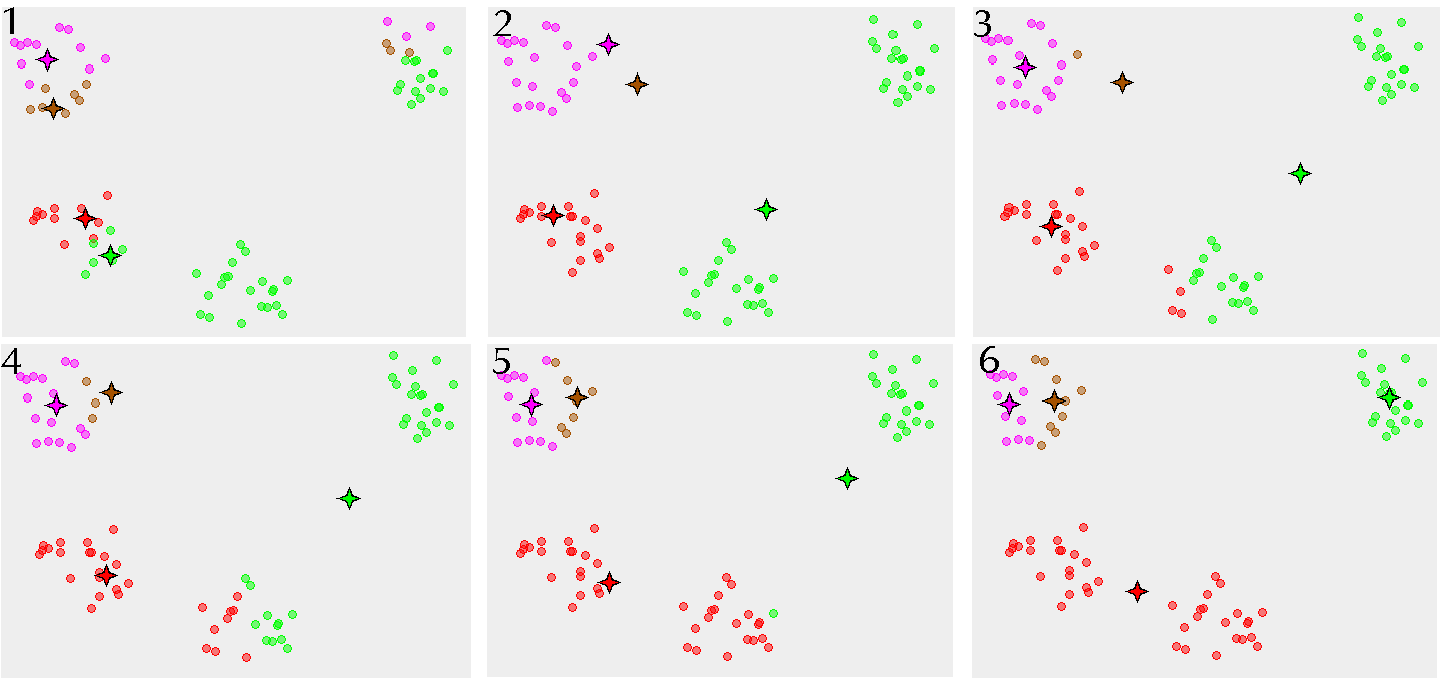
\includegraphics[width = \textwidth]{images/k-means-minimo-locale}
  \caption{K-Means converge in un minimo locale}
  \label{fig:k-means-minimo-locale}
\end{figure}

Abbiamo visto che uno dei punti delicati del \emph{k-means} è la scelta di $k$. Per capire quale sia il valore ottimo è possibile variare $k$ e \emph{plottare} i risultati. In particolare studieremo come varia  la \emph{Misura di Distorsione dei Cluster} in funzione di $k$, dove essa è definita come segue\footnote{A volte si usa la  \emph{Within Groups Sum of Squares} che è identica a $J(k)$ ma non normalizzata rispetto al numero di punti.}:
\begin{equation*}
J(k) = \frac{1}{N} \sum_{i=1}^N || x^{(i)} - \mu_c^{(i)} ||^2
\end{equation*}
in cui:
\begin{itemize}
\item $N$ è il numero complessivo di istanze;
\item $ x^{(i)}$ è la \emph{i-esima} istanza;
\item $\mu_c^{(i)}$ sono le coordinate del centroide del \emph{cluster} a cui appartiene $ x^{(i)}$;
\item $|| x^{(i)} - \mu_c^{(i)} ||^2$ è la distanza quadratica tra ciascuna istanza ed il suo centroide.
\end{itemize}
Ciò che ci interessa è minimizzare la somma delle distanze quadratiche, plottando $J$ in funzione di $k$. Un valore troppo alto di $J$ ci indica, ad esempio, che il \emph{clustering} non è significativo perché due o più \emph{cluster} potrebbero essere stati raggruppati attorno ad un unico centroide. Un valore troppo basso, però, è indice del fatto che abbiamo usato un numero troppo elevato di centroidi. Nel caso estremo avremo tanti centroidi quanti punti e questo porterà ad avere errore nullo. Tipicamente si può vedere che l'andamento di $J$ è decrescente (simile a quello in \autoref{fig:j(k)}) e si assume che il valore vero di $k$ coincida con il ginocchio di tale curva (cioè il punto in cui la pendenza comincia ad essere meno ripida, determinato tramite un'opportuna famiglia di algoritmi).

\begin{figure}[tbp]
\centering
  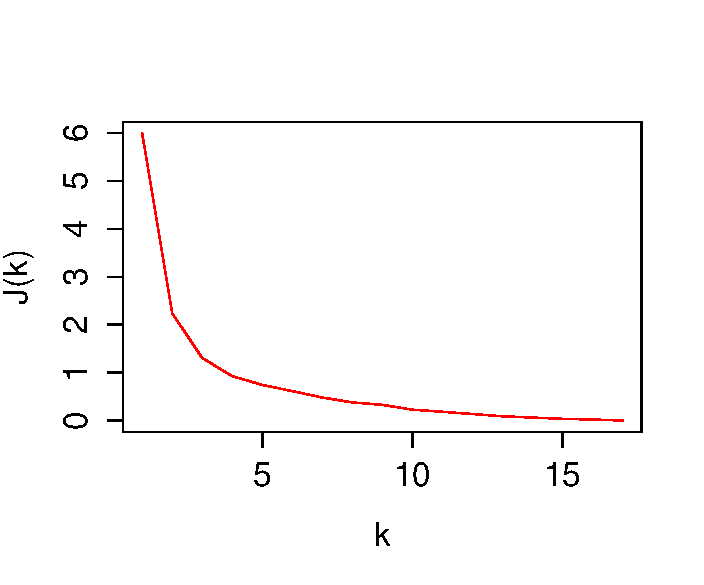
\includegraphics[width=0.7\textwidth]{images/jk}
  \caption{Andamento tipico della misura di distorsione dei cluster in funzione del numero di centroidi.}
  \label{fig:j(k)}
\end{figure}


\subsection{Principal Component Analysis}
\subsubsection{In sintesi}
Lo scopo di questa tecnica è passare da una rappresentazione delle istanze in $n$ variabili ad una rappresentazione in $p$ variabili \emph{latenti} (con $p<<n$). Nota bene che queste variabili sono \emph{latenti}, cioè non si tratta semplicemente di eliminare alcune \emph{feature} da quelle iniziali, ma di applicare un modello (lineare) alle \emph{feature} per \emph{proiettarle} in un nuovo dominio con dimensionalità inferiore. Questo nuovo dominio sarà caratterizzato da alcuni assi cartesiani, le coordinate di ciascun punto secondo il nuovo sistema di riferimento possono essere ottenute proiettando ciascun punto su ciascun asse. Le proiezioni dei punti su ciascun asse daranno luogo ad una distribuzione di valori e per ciascun asse è possibile calcolare la varianza di tale distribuzione. Poiché una varianza maggiore è indice del fatto che quella componente \emph{discrimina} maggiormente i punti, saremo interessati a prendere in considerazione solo le $p$ componenti a varianza maggiore (componenti principali). In questa maniera passiamo da una matrice degli ingressi di dimensione $m \times n$ ad una di dimensione $m \times p$. L'idea alla base delle tecniche di questo tipo è che le variabili osservabili siano in qualche maniera correlate e derivabili tutte da un insieme (più piccolo) di variabili latenti.

Capiamo meglio il concetto con un esempio. In~\autoref{fig:esempio_pca} sono mostrati alcuni punti, ciascuno dei quali è rappresentato da una coppia di valori $<x_1, x_2>$. La PCA ci consente di passare da una rappresentazione in $\mathcal{R}^2$ ad una rappresentazione in $\mathcal{R}$ (scegliendo $p=1$). Le componenti individuate dall'algoritmo (in seguito vedremo come) sono $u_1$ ed $u_2$. Proiettando i punti su $u_1$ ed $u_2$ ci rendiamo conto che la varianza delle proiezioni su $u_1$ è maggiore. Concludiamo che sarà questo asse la \emph{componente principale} ricercata e sarà sufficiente a descrivere il \emph{set} di istanze. In questo semplice esempio è facile capire che quanto fatto sia corretto, infatti tra $x_1$ ed $x_2$ sembra esserci una relazione lineare, e tra due variabili linearmente dipendenti è sufficiente conoscerne una per non perdere alcuna informazione (in questo caso la lineare dipendenza non è perfetta, quindi preserviamo gran parte dell'informazione, ma non tutta).

\begin{figure}[tbp]
\centering
  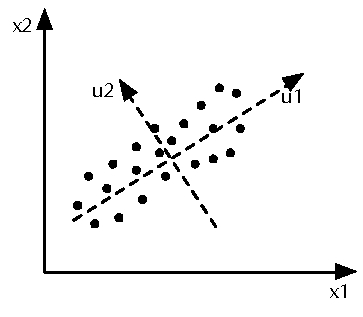
\includegraphics{images/esempio_pca}
  \caption{Esempio PCA}
  \label{fig:esempio_pca}
\end{figure}

\subsubsection{Passi necessari per la PCA}
Descriviamo quali passi sono necessari per portare a termine la PCA.

La prima operazione da fare è l'\emph{azzeramento del valor medio}, cioè a ciascuna \emph{feature}, di ciascuna istanza, sottraiamo il valor medio della stessa \emph{feature} calcolato su tutte le istanze. Passiamo quindi da
\begin{equation*}
x^{(i)}_1, x^{(i)}_2, \dots, x^{(i)}_n \qquad i = 1, \dots, m
\end{equation*}
a
\begin{equation*}
x^{(i)}_1 - \mu_1, x^{(i)}_2-\mu_2, \dots, x^{(i)}_n-\mu_n \qquad i = 1, \dots, m
\end{equation*}
con
\begin{equation*}
\mu_j = \frac{1}{m}\sum_{i=1}^m x^{(i)}_j.
\end{equation*}

Calcoliamo poi la matrice di covarianza ($\Sigma$) tra tutte le possibili coppie di \emph{feature}, il cui singolo elemento è così definito:
\begin{dmath*}
\Sigma_{ij} = \cov(x_i, x_j)
= E[(x_i-\mu_i)(x_j-\mu_j)]
= E[(x_i)( x_j)]
\end{dmath*}
Ricordiamo che la covarianza tiene conto di quanto due variabili aleatorie variano insieme, cioè di quanto sono simili nel loro comportamento.

Ora occorre conoscere autovalori ed autovettori della matrice delle covarianze. Per fare ciò applichiamo la \emph{Singular Value Decomposition} (SVD), anche nota come \emph{Decomposizione in Valori Singolari}, alla matrice $\Sigma$. Si tratta di una particolare fattorizzazione che, partendo da una matrice $A\in\mathbb{C}^{m\times n}$ ci consente di scrivere:
\begin{equation*}
A = U S V^*
\end{equation*}
dove:
\begin{itemize}
\item $U$ è una matrice unitaria sinistra di dimensioni $ m \times m$, cioè tale che moltiplicandola per la sua trasposta coniugata si ottiene la matrice identità ($U U^* = I$). Questa proprietà, nel caso di matrici reali, si traduce in $U^{-1} = U^T$;
\item $S$ è una matrice diagonale di dimensioni $m\times n$ (dove solo i primi $n$ elementi sono non nulli e costituiscono gli autovalori di A);
\item $V^*$ è la trasposta coniugata di una matrice unitaria di dimensioni $n\times n$.
\end{itemize}
Ricordiamo che la trasposta coniugata di una matrice si ottiene trasponendone gli elementi e sostituendo ciascuno di essi con il suo complesso coniugato (l'ordine delle due operazioni è irrilevante).

Gli elementi sulla diagonale principale di $S$ rappresentano gli autovalori di $A$, posti in ordine di valore decrescente man mano che ci si sposta verso il basso. Le colonne della matrice $U$  rappresentano gli autovettori sinistri di $A$ (cioè i vettori $\mathbf{u}$ t.c. $\mathbf{u}A=\mathbf{u}\lambda$ con $\lambda$ autovalore) e le colonne della matrice $V$ (e non $V^*$) rappresentano gli autovettori destri di $A$ (calcolati come $A\mathbf{v}=\lambda\mathbf{v} $). Nel caso di matrici simmetriche (come la matrice delle covarianze) questi autovalori coincidono, e quindi $U=V$. 

Ciò che si fa nel caso della PCA è applicare la SVD alla matrice delle covarianze:
\begin{equation*}
\Sigma = U S V^*
\end{equation*}
a questo punto di tutti gli autovalori che compaiono in $S$ ci interessa conservare solo i primi $p$, per questi autovalori consideriamo i corrispondenti autovettori. Ciascun autovettore sarà costituito da $n$ elementi, avremo quindi una matrice degli autovettori di dimensione $n \times p$.
Moltiplicare la matrice degli ingressi per l'autovettore \emph{i-esimo} significa calcolare il valore della coordinata \emph{i-esima} di ciascun ingresso rispetto al nuovo sistema di riferimento. Quindi moltiplicare la matrice degli ingressi ($m \times n$) per l'intera matrice degli autovettori ($n \times p$) equivale ad effettuare il cambio di coordinate richiesto per tutti gli ingressi. Il risultato sarà la nuova matrice dei campioni di dimensione ridotta ($m \times p$).

\begin{figure}
\centering
\begin{subfigure}[b]{0.5\textwidth}
\centering
  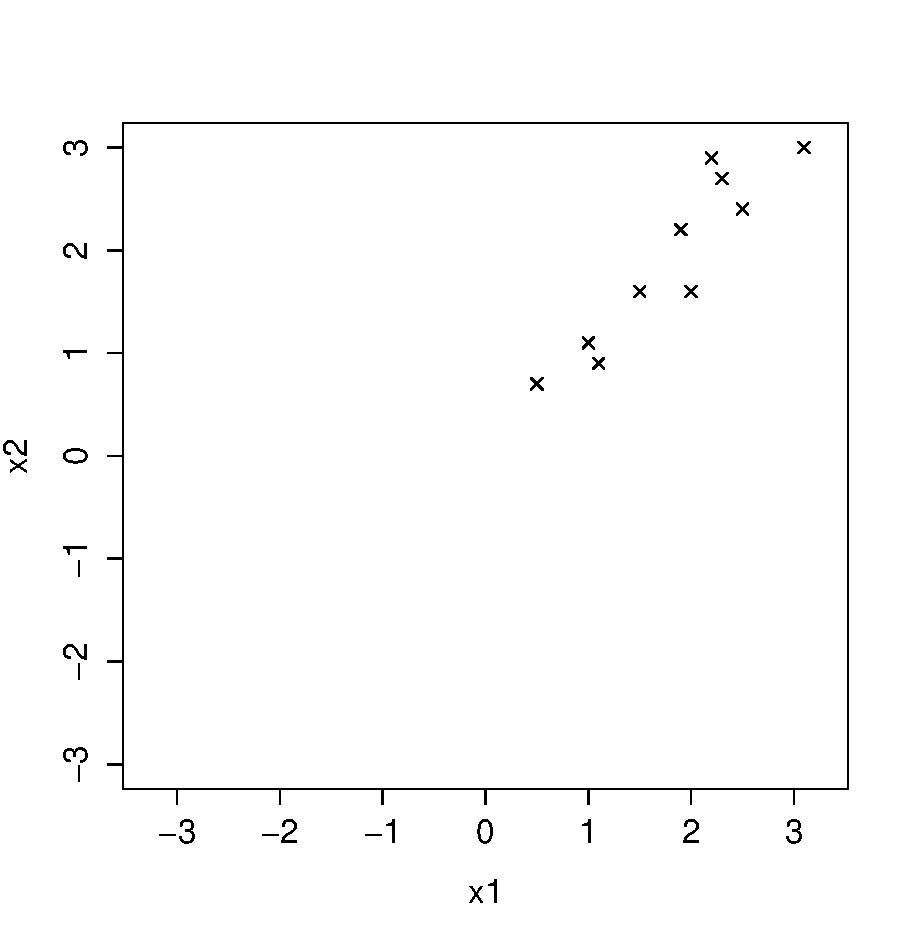
\includegraphics[width=\columnwidth]{images/points}
  \caption{Punti iniziali}
  \label{fig:punti_iniziali}
\end{subfigure}%
\begin{subfigure}[b]{0.5\textwidth}
    \centering
  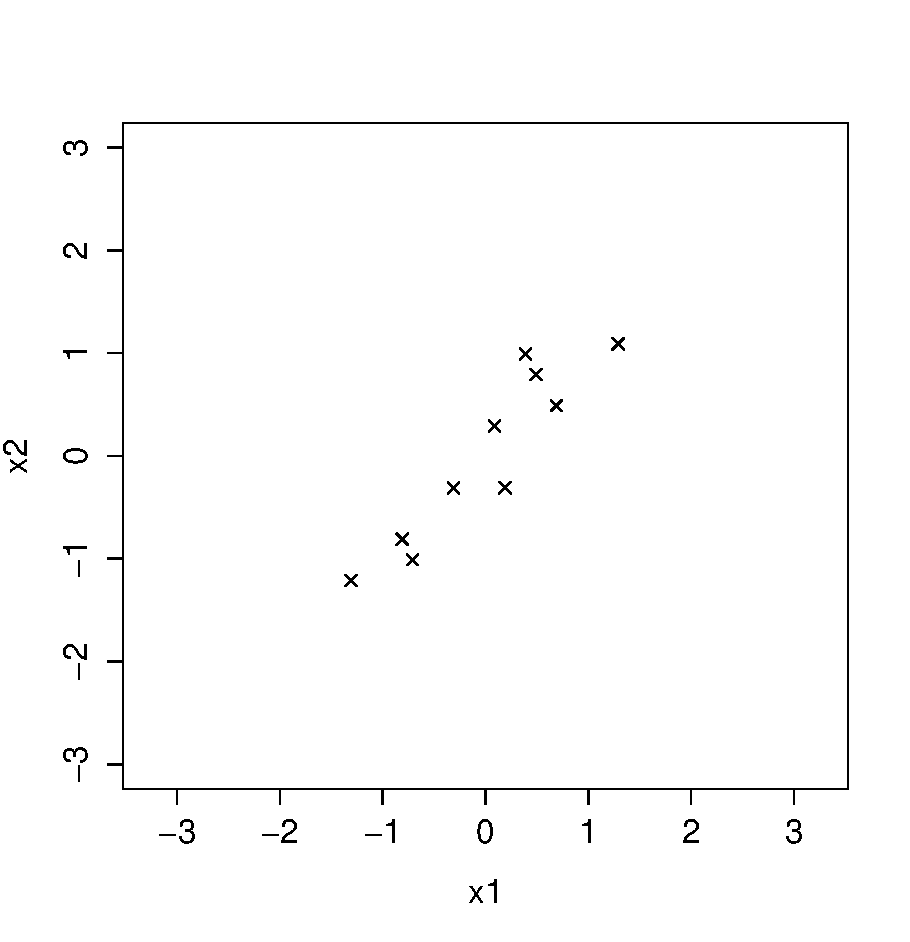
\includegraphics[width=\columnwidth]{images/points_scaled}
  \caption{Punti con media azzerata}
  \label{fig:punti_scalati}
\end{subfigure}
\caption{Campioni a cui applicare la PCA }
\label{fig:PCA}
\end{figure}



\begin{esempio}
Chiariamo la procedura tramite un esempio numerico\footnote{Esempio trattato a lezione e preso da \href{http://www.cs.otago.ac.nz/cosc453/student_tutorials/principal_components.pdf}{qui}.} eseguito in R. I dati a disposizione sono rappresentati dalle seguenti coppie di punti (\autoref{fig:punti_iniziali}):
\begin{lstlisting}
> show (dataset)
    x1  x2
1  2.5 2.4
2  0.5 0.7
3  2.2 2.9
4  1.9 2.2
5  3.1 3.0
6  2.3 2.7
7  2.0 1.6
8  1.0 1.1
9  1.5 1.6
10 1.1 0.9
\end{lstlisting} 
Eseguiamo ora i passi della PCA:
\begin{enumerate}
\item \emph{Azzeramento della media}, che effettuiamo tramite la funzione \texttt{scale}, per ottenere la nuova matrice degli ingressi con le medie azzerate (mostrati in \autoref{fig:punti_scalati}):
\begin{lstlisting}
> scaled.dataset <- scale(dataset, TRUE, FALSE)
> show(scaled.dataset)
         x1    x2
 [1,]  0.69  0.49
 [2,] -1.31 -1.21
 [3,]  0.39  0.99
 [4,]  0.09  0.29
 [5,]  1.29  1.09
 [6,]  0.49  0.79
 [7,]  0.19 -0.31
 [8,] -0.81 -0.81
 [9,] -0.31 -0.31
[10,] -0.71 -1.01
\end{lstlisting}

\item \emph{Calcolo della matrice delle covarianze}:
\begin{lstlisting}
>  Sigma <- cov(scaled.dataset)
>  show(Sigma)
          x1        x2
x1 0.6165556 0.6154444
x2 0.6154444 0.7165556
\end{lstlisting}

\item \emph{Decomposizione ai valori singolari}:
 \begin{lstlisting}
> results <- svd(Sigma)
>  show(results)
$d
[1] 1.2840277 0.0490834

$u
           [,1]       [,2]
[1,] -0.6778734 -0.7351787
[2,] -0.7351787  0.6778734

$v
           [,1]       [,2]
[1,] -0.6778734 -0.7351787
[2,] -0.7351787  0.6778734
\end{lstlisting}

Notiamo che l'\emph{output} è costuito da un vettore e due matrici. Il vettore (\texttt{d}) contiene i due autovalori (è la diagonale principale di $S$), mentre le matrici (\texttt{u} e \texttt{v}) contengo rispettivamente gli autovettori sinistri e destri, uno per colonna, e corrispondono quindi ad $U$ e $V$ (non $V^*$). Notiamo anche che, essendo $\Sigma$ reale, accade che $u = v$.

\item \emph{Proiezione dei dati sul nuovo sistema di riferimento}. Volendo ridurre il numero di \emph{feature} da $2$ ad $1$, ci limitiamo a considerare l'autovalore più grande (il primo) ed il corrispondente autovettore (la prima colonna di \texttt{u} o \texttt{v}).
A questo punto moltiplichiamo la matrice dei campioni per questo autovettore ed otteniamo le coordinate dei punti nel nuovo spazio:
\begin{lstlisting}
> new.dataset <- scaled.dataset %*% results$u[,1] 
> show(new.dataset)
             [,1]
 [1,] -0.82797019
 [2,]  1.77758033
 [3,] -0.99219749
 [4,] -0.27421042
 [5,] -1.67580142
 [6,] -0.91294910
 [7,]  0.09910944
 [8,]  1.14457216
 [9,]  0.43804614
[10,]  1.22382056
\end{lstlisting}



\end{enumerate}

A questo punto la PCA è conclusa ma, poiché stiamo lavorando con punti del piano, possiamo visualizzare graficamente quali siano le due componenti individuate. Per disegnare ciascuna componente è sufficiente sovrappore al \emph{plot} dei punti (scalati) la retta con intercetta nulla e coefficiente angolare pari al rapporto tra il primo ed il secondo elemento dell'autovettore (equivalentemente si potrebbero usare i punti iniziali e \emph{plottare} questa retta con le coordinate traslate di una quantità pari alle medie sottratte in partenza).
\begin{lstlisting}
plot(scaled.dataset, pch = 4, xlim = c(-3,3), ylim = c(-3,3))

m1 <-  results$u[,1][1] / results$u[,1][2] 
comp1 <- matrix(c(seq(-3,3), m1*seq(-3,3)), 7, 2)
points(comp1, col="red", type = "l")

m2 <-  results$u[,2][1] / results$u[,2][2] 
comp2 <- matrix(c(seq(-3,3), m2*seq(-3,3)), 7, 2)
points(comp2, col="blue", type = "l" )
\end{lstlisting}
Il risultato è mostrato in \autoref{fig:components_scaled}. Effettivamente notiamo che le proiezioni dei punti sulla prima componente (quella disegnata in rosso) hanno varianza maggiore. Verifichiamo se quest'ultima affermazione è vera calcolando le varianze delle proiezioni dei punti sui due assi:
\begin{lstlisting}
> var(scaled.dataset %*% results$u[,1])
         [,1]
[1,] 1.284028
> var(scaled.dataset %*% results$u[,2])
          [,1]
[1,] 0.0490834
\end{lstlisting}
Questi risultati confermano quanto ci aspettavamo e notiamo che la varianza lungo ciascuna componente è pari proprio all'autovalore che determina tale componente (motivo per cui consideriamo gli autovalori più grandi).

\begin{figure}[tbp]
\centering
  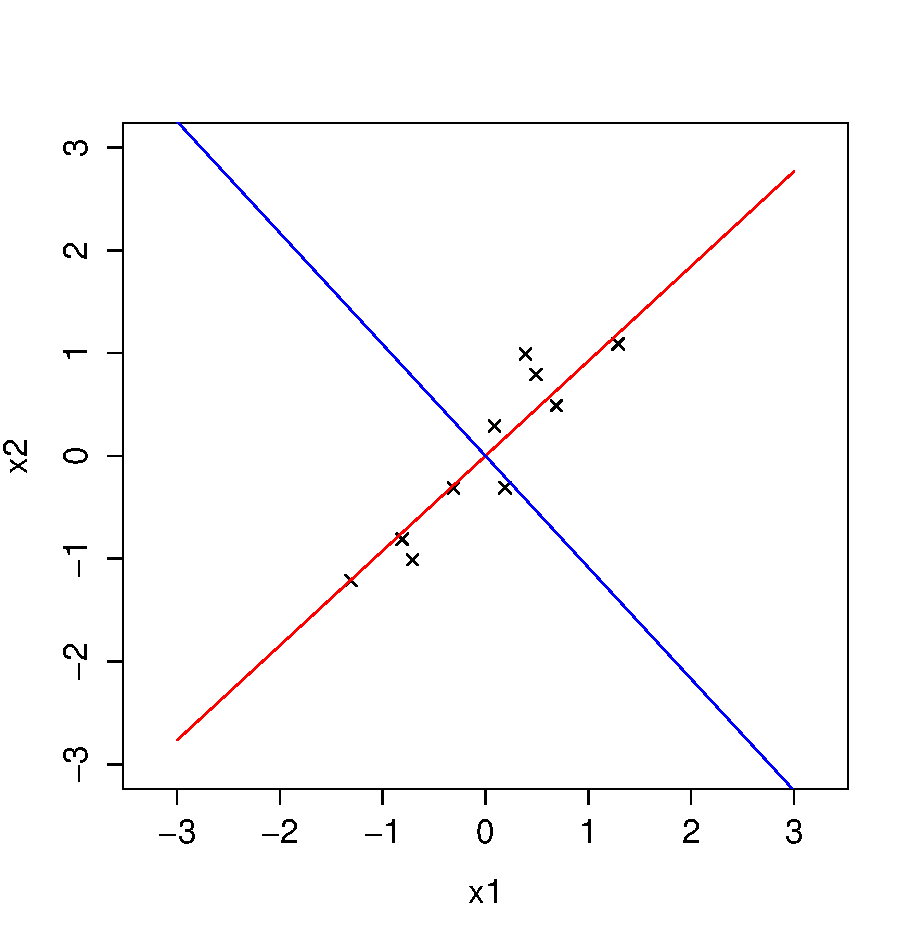
\includegraphics[width=0.5\textwidth]{images/components_scaled}
  \caption{Componenti individuate tramite PCA}
  \label{fig:components_scaled}
\end{figure}
\end{esempio}

\clearpage
\subsection{Soft clustering tramite GMM}

In questo capitolo esamineremo i \emph{mixture model}. Si tratta di modelli probabilistici, cioè di funzioni densità di probabilità, ottenuti dalla somma pesata di densità di probabilità elementari. In particolare ci occuperemo di \emph{Gaussian Mixture Model} (GMM) cioè di modelli probabilistici ottenuti dalla somma pesata di un certo numero di funzioni gaussiane. L'ambito in cui applicheremo le GMM è il \emph{soft clustering}, cioè esamineremo una procedura, basata sull'utilizzo di GMM, che sia in grado di dirci qual è la probabilità che un punto appartenga a ciascun \emph{cluster} individuato in una nuvola di punti.


\begin{figure}[h]
\centering
\begin{subfigure}[b]{0.5\textwidth}
    \centering
    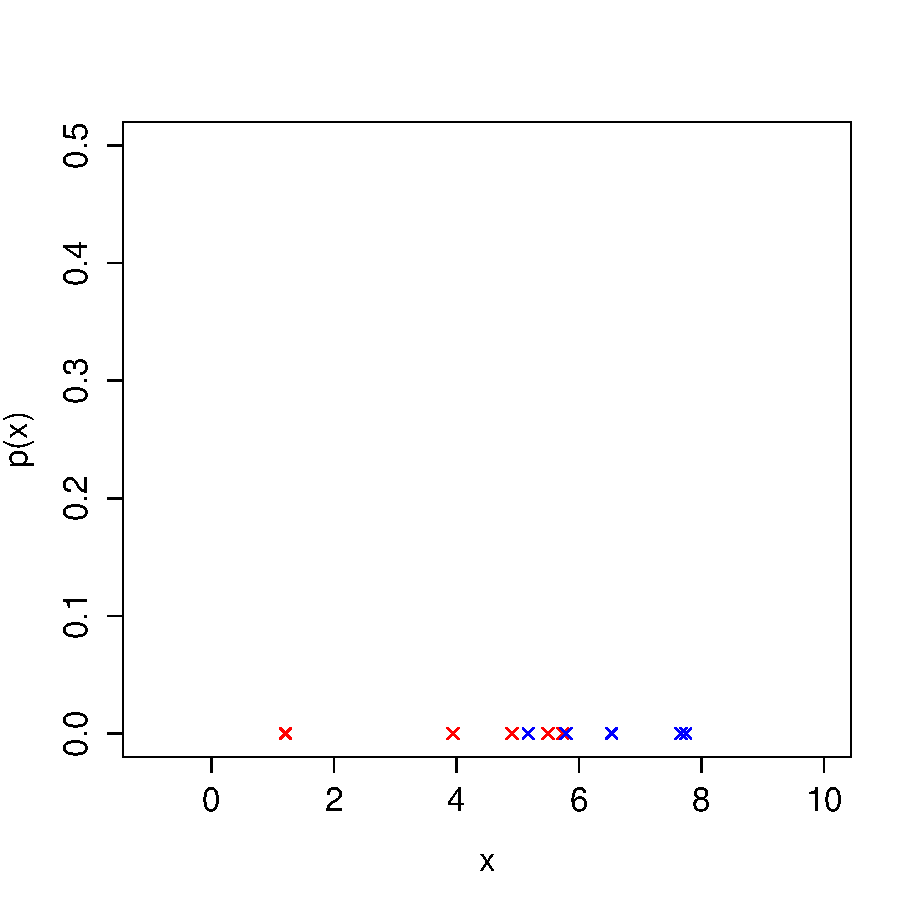
\includegraphics[width=\columnwidth]{images/gmm_points}
    \caption{}
    \label{fig:gmm_points}
\end{subfigure}%
\begin{subfigure}[b]{0.5\textwidth}
    \centering
    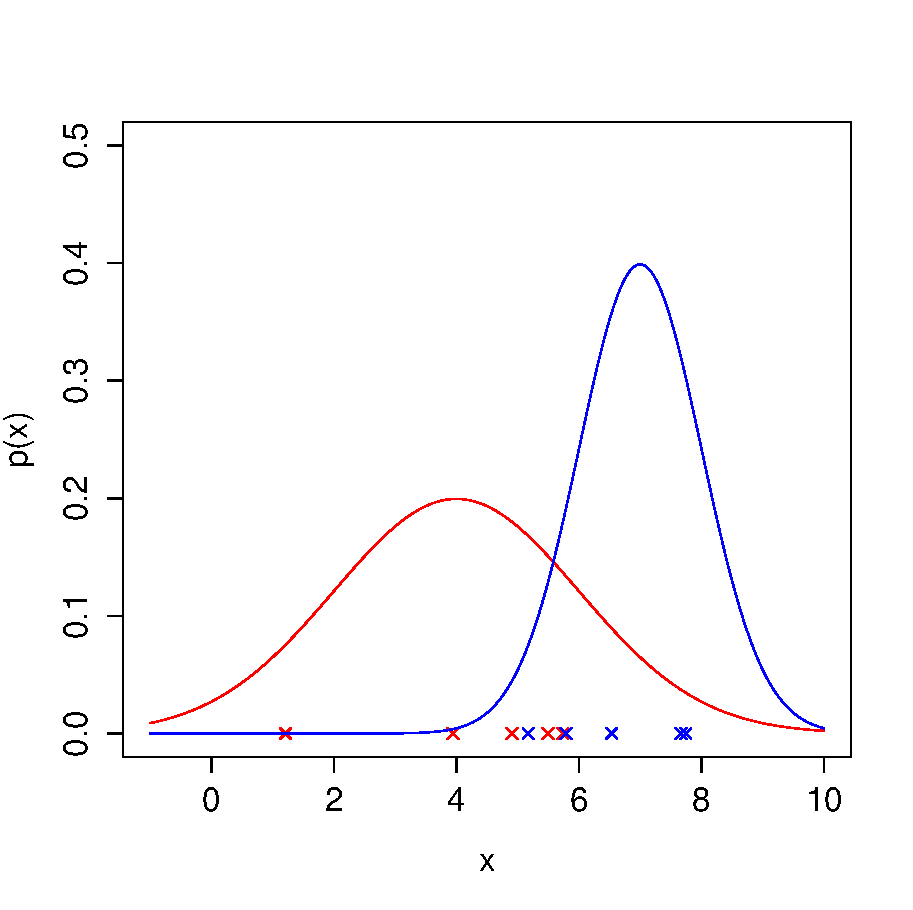
\includegraphics[width=\columnwidth]{images/gmm_gaussians}
    \caption{}
    \label{fig:gmm_gaussians}
\end{subfigure}
\caption{Punti da \emph{clusterizzare} e gaussiane da cui sono stati estratti.}
\label{fig:gmm_example}
\end{figure}


\subsubsection{L'idea in sintesi}
Per capire l'approccio adottato partiamo da un semplice esempio. Ipotizziamo di voler effettuare il \emph{clustering} di un certo numero di punti caratterizzati da una sola coordinata. Essi sono rappresentabili su una retta, come mostrato sull'asse $x$ in \autoref{fig:gmm_points}. Per comodità i punti di ciascun \emph{cluster} sono rappresentati con un colore differente. Ipotizziamo che i punti appartenenti a ciascun \emph{cluster} siano distribuiti come se fossero stati estratti da una gaussiana. Quindi, nel nostro esempio, avremo due gaussiane con parametri diversi tra di loro (\autoref{fig:gmm_gaussians}). Se riuscissimo a determinare tali parametri, saremmo in grado di calcolare la probabilità che un nuovo punto sia stato generato dalla prima o dalla seconda gaussiana. Ciò significherebbe conoscere la probabilità che il punto appartenga al primo \emph{cluster} e la probabilità che appartenga al secondo \emph{cluster}, ovvero avremmo realizzato \emph{soft clustering}.

Per determinare i parametri delle due gaussiane operiamo direttamente sul GMM corrispondente, cioè stiamo ipotizzando che i punti da \emph{clusterizzare} siano stati generati da un GMM. In prima analisi potremmo immaginarlo come la somma delle due gaussiane, così come mostrato dalla linea tratteggiata in \autoref{fig:gmm_gmm}. Tuttavia sorge un problema: come ben noto l'area sottesa da ciascuna gaussiana è unitaria, quindi l'area sottesa dalla loro somma non lo sarà. Affinché il GMM sia un modello probabilistico, ovvero affinché sia una densità di probabilità, è necessario che sottenda anch'esso un'area unitaria. Per tale motivo ciascuna delle gaussiane di partenza viene moltiplicata per una quantità compresa tra $0$ ed $1$ prima di essere sommata alle altre. Intuitivamente questo giustifica il fatto che un GMM sia una somma pesata di distribuzioni elementari. Vedremo in seguito che significato fisico è possibile dare a questi pesi.

\begin{figure}[tbp]
\centering
  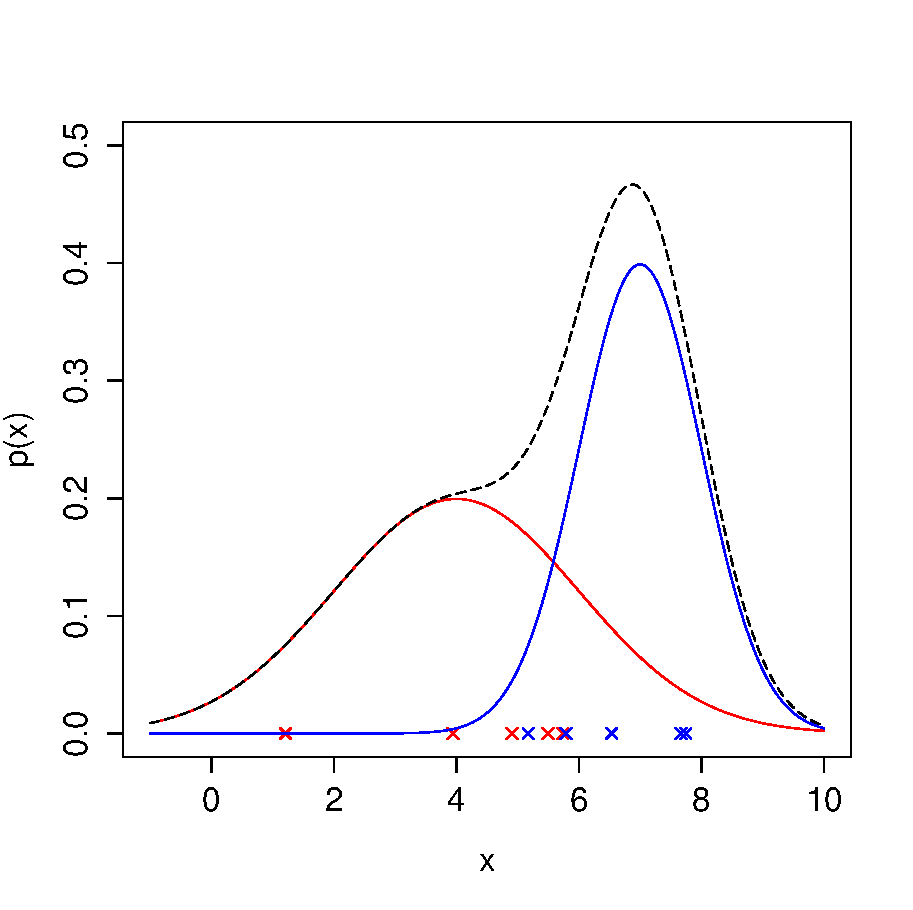
\includegraphics[width = 0.5\columnwidth]{images/gmm_gmm}
  \caption{Somma delle due gaussiane.}
  \label{fig:gmm_gmm}
\end{figure}


Il caso esaminato fin qui prevede che ciascun punto sia descritto da una sola coordinata. Nel caso di punti a $2$ o più variabili l'idea di fondo rimane invariata, mentre cambiano alcuni dettagli. In particolare non potremo più usare una semplice distribuzione gaussiana univariata, ma dovremo ricorrere ad una gaussiana multivariata. Nel caso in cui i punti da \emph{clusterizzare} si trovino sul piano ($n=2$) la mistura di gaussiane assume una forma simile a quella mostrata in \autoref{fig:esempio_GMM}. In essa è rappresentato un GMM formato da $3$ distribuzioni gaussiane bidimensionali (o bivariate).



\begin{figure}[tbp]
\centering
  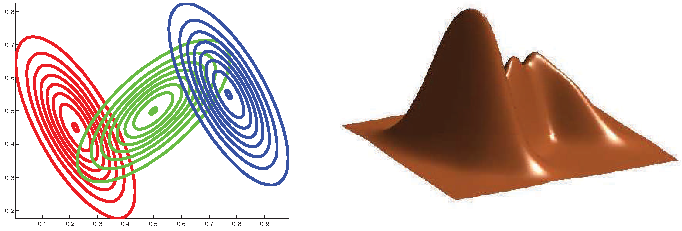
\includegraphics[width = 0.8\textwidth]{images/esempio_GMM}
  \caption{Esempio di GMM con 3 gaussiane bivariate}
  \label{fig:esempio_GMM}
\end{figure}

\subsubsection{Dettagli matematici}
Nei paragrafi che seguono formalizziamo meglio il problema ed approfondiamo alcuni dettagli. 

\paragraph{Mixture model in formule}
Fin qui abbiamo definito una mistura di gaussiane come una somma pesata di densità di probabilità gaussiane. Più in generale possiamo parlare di \emph{Mixture Model} come una somma pesata di densità di probabilità, senza specificarne la natura. Ipotizzando di voler creare una mistura con $k$ componenti, la formulazione più generica per la densità di probabilità del modello è\footnote{Per una formulazione più formale vedi \href{http://www.youtube.com/watch?v=Rkl30Fr2S38}{qui}.}:

\begin{equation*}
p(\mathbf{x}) = \sum_{j=1}^k p(\mathbf{x} \land z = j).
\end{equation*}
Nella precedente $p(\mathbf{x} \land z = j)$ rappresenta la probabilità che il punto $\mathbf{x}$ sia stato generato dalla \emph{j-esima} componente. Applicando la regola del prodotto possiamo riscriverla nella formulazione tipicamente usata:
\begin{equation*}
p(\mathbf{x}) = \sum_{j=1}^k p(\mathbf{x}| z = j) p(z = j).
\end{equation*}
In essa $z$ rappresenta una variabile casuale discreta (latente) che assume valori da $1$ a $k$. $p(z=j)$ indica la probabilità che la \emph{j-esima} componente della mistura venga ``attivata'' e generi il campione.
A livello intuitivo possiamo pensare al processo di generazione di un punto in questa maniera:
\begin{itemize}
\item la componente \emph{j-esima} viene selezionata per la generazione del punto con una probabilità $p(z=j)$;
\item il punto viene generato dalla componente \emph{j-esima} con una probabilità $p(\mathbf{x}|z=j)$ che dipende \emph{solo} dalla natura di questa componente (cioè dalla sua specifica distribuzione di probabilità).
\end{itemize}
In definitiva, possiamo vedere la precedente formula come una risposta alla domanda:
\begin{itemize}
\item ``Con quale probabilità la mistura può generare un punto $\mathbf{x}$?''
\end{itemize}
La risposta fornita dalla formula è:
\begin{itemize}
\item ``Per ciascuna distribuzione, considera la probabilità che sia essa a generare quel punto e moltiplicala per la probabilità con cui essa lo genererebbe. In seguito somma tutte queste quantità e saprai con che probabilità la mistura darà vita al punto $\mathbf{x}$.''
\end{itemize}

A questo punto possiamo semplificare la notazione introducendo i coefficienti $\pi_j = p(z=j)$ che ci consentono di scrivere: 
\begin{equation*}
p(\mathbf{x}) = \sum_{j=1}^k \pi_j p_j(\mathbf{x}).
\end{equation*}
$p_j(\mathbf{x}$) rappresenta la densità di probabilità della \emph{j-esima} componente calcolata nel punto $\mathbf{x}$, mentre i vari $\pi_j$ prendono il nome di \emph{mixing coefficients} e sono proprio i pesi di cui abbiamo parlato finora. Notiamo anche che, trattandosi di valori di probabilità, la loro somma è unitaria:
\begin{equation*}
\sum_{j=1}^k\pi_j= \sum_{j=1}^k p(z=j) = 1.
\end{equation*}

Poiché il nostro scopo sarà individuare i parametri migliori per le singole distribuzioni, conviene adottare una notazione più esplicita, cioè la seguente:

\begin{equation*}
p(\mathbf{x}|\boldsymbol{\theta}) = \sum_{j=1}^k \pi_j p_j(\mathbf{x} | \boldsymbol{\theta_j})
\end{equation*}
in cui $\boldsymbol\theta_j$ rappresenta i parametri della componente \emph{j-esima}, ad esempio media e varianza di una gaussiana univariata, mentre $\boldsymbol\theta$ è una particolare istanza di tutti i parametri $\boldsymbol\theta_j$.

\paragraph{Parametri di un GMM}
Fin qui abbiamo parlato genericamente di ``parametri'' di un modello. Scendiamo ora nel dettaglio delle GMM. Il primo passo da fare è sostituire la generica densità di probabilità $p_j(\mathbf{x} | \boldsymbol{\theta_j})$ con la \emph{j-esima} gaussiana multivariata, la cui espressione è:

\begin{equation*}
\mathcal{N}(\mathbf{x} | \boldsymbol{\mu_j}, \boldsymbol{\Sigma_j}) = \frac{1}{\sqrt{(2\pi)^{n} |\boldsymbol\Sigma_j|}} \exp\left(-\frac{1}{2}({\mathbf x}-{\boldsymbol\mu_j})^T{\boldsymbol\Sigma_j}^{-1}({\mathbf x}-{\boldsymbol\mu_j})
\right)
\end{equation*}
nella quale:
\begin{itemize}
\item $n$ rappresenta la dimensione di ciascun ingresso (e quindi il numero di \emph{feature});
\item $\boldsymbol\mu_j$ è il vettore dei valori medi della \emph{j-esima} gaussiana;
\item $\boldsymbol\Sigma_j$ è la matrice delle covarianze della \emph{j-esima} gaussiana.
\end{itemize}
I parametri che desideriamo individuare sono quindi:
\begin{gather*}
\boldsymbol\mu_j \text{~e~} \boldsymbol\Sigma_j \quad j=1, \dots, k.
\end{gather*}

Nel caso di gaussiane univariate questi si riducono ai valori medi ($\mu_j$) ed alle varianze ($\sigma^2_j$). Se per ogni \emph{cluster} sapessimo quali punti appartengono ad esso, potremmo calcolare le stime di media e varianza tramite le formule note:
\begin{gather*}
\hat\mu_j = \frac{1}{|C_j|} \sum_{ x^{(i)} \in C_j} x^{(i)} \\
\hat\sigma^2_j = \frac{1}{|C_j|-1} \sum_{x^{(i)} \in C_j}(x^{(i)}- \hat\mu_j)^2
\end{gather*}
dove ${C_j}$ rappresenta il \emph{j-esimo} \emph{cluster} e $|{C_j}|$ è il numero di punti di cui è composto. Chiaramente lo stesso discorso può essere esteso al caso multivariato:
\begin{gather*}
\boldsymbol{\hat\mu_j} = \frac{1}{|C_j|} \sum_{ \mathbf{x^{(i)}} \in C_j} \mathbf{x^{(i)}} \\
\hat\Sigma_j = \frac{1}{|C_j|-1} \sum_{\mathbf{x^{(i)}} \in C_j}(\mathbf{x^{(i)}}- \boldsymbol{\hat\mu_j})(\mathbf{x^{(i)}}- \boldsymbol{\hat\mu_j})^T
\end{gather*}
Purtroppo, però, non è noto a priori quali punti siano stati generati da ciascun cluster, altrimenti il problema del \emph{clustering} non si porrebbe neppure. Potremmo quindi pensare di assegnare ciascun punto ad un \emph{cluster} in base alla gaussiana a cui appartiene con maggiore probabilità. Fare ciò, tuttavia, richiederebbe di conoscere i parametri delle gaussiane, che non sono affatto noti. Ci troviamo quindi in questa situazione:
\begin{itemize}
\item per stimare i parametri di ciascuna gaussiana dovremmo conoscere i punti che le appartengono;
\item per conoscere i punti che appartengono a ciascuna gaussiana dovremmo stimarne i parametri.
\end{itemize}
La procedura che risolve questo problema si chiama \emph{Expectation-Maximization} (EM).

\paragraph{Algoritmo EM per GMM}

L'algoritmo EM applicato ad un GMM può essere sintetizzato nei seguenti passaggi\footnote{I dettagli sulle formule sono in ``Machine Learning - A Probabilistic Perspective'', Sezione 11.4.2}:
\begin{enumerate}
    \item fissato $k$ inizializza casualmente i parametri delle gaussiane ed i pesi $\pi_j$;
    \item passo E (\emph{Expectation}): per ogni coppia punto-\emph{cluster} calcola alcuni coefficienti, detti \emph{responsibility}, definiti come segue:
        \begin{equation*}
r_{ij}\triangleq p(z=j | \mathbf{x^{(i)}}, \boldsymbol\theta^{t-1})
        \end{equation*}
 dove $\boldsymbol\theta^{t-1}$ rappresenta i parametri del modello all'iterazione precedente. Ciascun coefficiente tiene conto di quanto il \emph{cluster} \emph{j-esimo} sia responsabile del punto \emph{i-esimo} ed è calcolato come il rapporto tra la probabilità che il punto sia stato generato dal \emph{cluster} e quella che sia stato generato dall'intero GMM:
         \begin{equation*}
r_{ij} =\frac{\pi_j p_j(\mathbf{x}^{(i)} | \boldsymbol{\theta_j}^{(t-1)})}{ \sum_{j=1}^k \pi_j p_j(\mathbf{x}^{(i)}  | \boldsymbol{\theta_j}^{(t-1)})}
         \end{equation*}
    \item passo M (\emph{Maximization}): per ogni gaussiana ricalcola i parametri $\pi_j$, $\boldsymbol\mu_j$ e $\boldsymbol\Sigma_j$ in base alle \emph{responsibility} appena calcolate, con lo scopo di massimizzare la \emph{likelihood} (cioè la probabilità che quei punti siano stati generati dal GMM):
        \begin{gather*}
            \pi_j = \frac{1}{m} \sum_{i=1}^m r_{ij} \\
           \boldsymbol{\mu_j} = \frac{\sum_{i} r_{ij}\mathbf{x^{(i)}}}{\sum_{i} r_{ij}} \\
            \mathbf{\Sigma_j} = \frac{\sum_{i} r_{ij} (\mathbf{x}^{(i)} - \boldsymbol{\mu_j})(\mathbf{x}^{(i)} - \boldsymbol{\mu_j})^T} {\sum_{i} r_{ij}}
    \end{gather*}
\item ripeti i passi E ed M fino a convergenza.
\end{enumerate}

%Come già accennato, l'idea dei modelli basati su variabili latenti è che l'insieme di variabili osservabili sia deducibile a partire da un insieme più piccolo di variabili latenti\footnote{Machine Learning - A Probabilistic Perspective, Capitolo 11}. Se chiamiamo $z_i$ le variabili latenti ed $x_i$ quelle osservabili possiamo distinguere i seguenti modelli:
%\begin{itemize}
%\item \emph{molti a molti}, in cui ciascuna variabile latente influisce su più variabili osservabili e ciascuna variabile osservabile subisce l'influenza di più variabili latenti;
%\item \emph{uno a molti}, in cui una variabile latente influisce su più variabili osservabili;
%\item \emph{molti ad uno}, in cui più variabili latenti influiscono su una singola variabile osservabile;
%\item \emph{uno ad uno}, in cui una variabile latente influisce su una sola variabile osservabile.
%
%\end{itemize}
%\begin{figure}[tbp]
%\centering
%  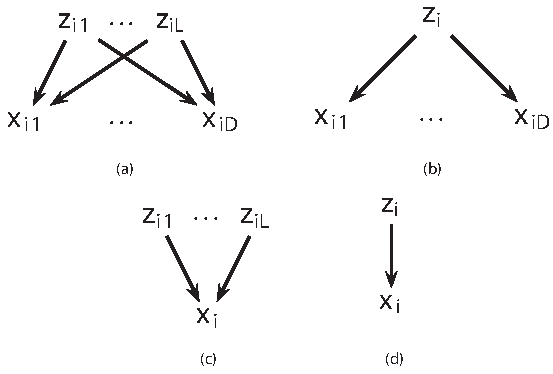
\includegraphics[width = 0.6\textwidth]{images/cardinalita_modelli_latenti}
%  \caption{Possibili cardinalità della relazione $z_i \rightarrow x_i$}
%\label{fig:cardinalita_modelli_latenti}
%\end{figure}
%
%Assumendo che $\mathbf{x_i}$ e $\mathbf{z_i}$ possano essere vettori, la notazione $\mathbf{z_i} \rightarrow\mathbf{x_i}$ riassume tutti i casi precedenti. A questo punto possiamo definire:
%\begin{itemize}
%\item $p(\mathbf{x_i}| \mathbf{z_i})$ come la probabilità che un'istanza di variabili osservabili $\mathbf{x_i}$ venga generata a partire da un'istanza di variabili latenti $\mathbf{z_i}$ (detta \emph{likelihood});
%\item $p(\mathbf{z_i})$ probabilità a priori delle variabili latenti.
%\end{itemize}
%A seconda della scelta delle due distribuzioni si possono generare diversi modelli.

%\subsection{Forma generale}
%Una forma generale e semplice per descrivere un \emph{mixture model} è questa\footnote{Vedi anche AIMA, Capitolo 20.3.}:
%\begin{equation*}
%p(\mathbf{x_i}|\theta) = \sum_{k=1}^K \pi_k p_k(\mathbf{x_i}|\theta)
%\end{equation*}
%in cui:
%\begin{itemize}
%\item $p(\mathbf{x_i}|\theta)$ rappresenta la probabilità che i dati a disposizione $\mathbf{x_i}$ vengano generati da un modello probabilistico i cui parametri sono $\theta$;
%\item $K$ rappresenta il numero di possibili stati latenti (discreti), che nel caso del \emph{clustering} corrisponderà al numero di \emph{cluster};
%\item $\pi_k$ sono dei coefficienti numerici che fungono da pesi, tali che $0\leq\pi_k\leq1$ e $\sum_k(\pi_k)=1$, se pensiamo all'estrazione di un punto dal modello possiamo vederli come la probabilità che un campione venga generato a partire dalla \emph{k-esima} componente della mistura;
%\item $ p_k(\mathbf{x_i}|\theta)$ rappresenta la distribuzione di probabilità del \emph{k-esimo} stato latente, fissati i parametri $\theta$.
%\end{itemize}
%
%Applicando questo modello al \emph{clustering} (\emph{soft clustering} per l'esattezza) stiamo facendo ciò: ipotizziamo che siano presenti $K$ \emph{cluster},  ciascuno di essi è rappresentato da una densità di probabilità. Per ciascun campione calcoliamo la probabilità che esso appartenga a ciascun cluster, cioè a ciascuna distribuzione di probabilità (\emph{responsibility}), e qui terminerebbe il \emph{clustering}. Per capire il significato dell'espressione precedente, consideriamo che, intuitivamente, sommando le probabilità appena descritte otterremmo la probabilità che quel campione sia stato assegnato con un certo grado di certezza ad almeno un \emph{cluster}. Tuttavia la somma sarebbe maggiore di 1, e non potrebbe rappresentare una probabilità essa stessa, quindi facciamo una somma pesata secondo i coefficienti $\pi_k$. 
%
%Quindi, se accade che $p(\mathbf{x_i}|\theta)$ è piccolo, signfica che non c'è alcun \emph{cluster}  al quale si può ``scommettere'' che l'istanza appartenga, perché mediamente esso appartiene a ciascun \emph{cluster} con una probabilità molto bassa. L'ideale si ha quando la somma di queste probabilità su tutte le istanze è alta, cioè quando bene o male per ciascun campione ho individuato uno o più \emph{cluster} a cui esso appartiene ``abbastanza probabilmente''.
%
%\subsection{Gaussian Mixture Model}
%Nel caso di GMM la probabilità che un punto appartenga a ciascun \emph{cluster} è gaussiana multivariata (cioè in più dimensioni), dall'espressione:
%\begin{equation*}
%\mathcal{N}(\mathbf{x}_i|\boldsymbol{\mu}_k, \boldsymbol\Sigma_k) = \frac{1}{\sqrt{(2\pi)^{D} |\boldsymbol\Sigma_k|}} \exp\left(-\frac{1}{2}({\mathbf x_i}-{\boldsymbol\mu_k})^T{\boldsymbol\Sigma_k}^{-1}({\mathbf x_i}-{\boldsymbol\mu_k})
%\right)
%\end{equation*}
%in cui:
%\begin{itemize}
%\item $D$ rappresenta la dimensione di ciascun ingresso (e quindi il numero di dimensioni della gaussiana);
%\item $\boldsymbol\mu_k$ il vettore dei valor medi della \emph{k-esima} gaussiana;
%\item $\boldsymbol\Sigma_k$ la matrice delle covarianze della \emph{k-esima} gaussiana.
%\end{itemize}
%Il modello GMM è quindi:
%\begin{equation*}
%p(\mathbf{x_i}|\theta) = \sum_{k=1}^K \pi_k \mathcal{N}(\mathbf{x}_i|\boldsymbol{\mu}_k, \boldsymbol\Sigma_k).
%\end{equation*}
%In~\autoref{fig:esempio_GMM} è mostrato un esempio grafico di come può apparire il modello con $k=3$ e $D=2$.
%
%
%
%Il problema in tutto ciò è come determinare i parametri $\boldsymbol\mu_k$ e $\mathbf\Sigma_k$ per ciascuna gaussiana quando facciamo \emph{clustering}. Infatti a priori non abbiamo informazioni a sufficienza, ovvero:
%\begin{itemize}
%\item per determinare la probabilità con cui ciascun punto appartiene a ciascuna gaussiana dovremmo conoscere i parametri delle gaussiane;
%\item per determinare i parametri delle gaussiane dovremmo sapere quali punti appartengono a ciascuna di esse.
%\end{itemize}
%


\subsection{Outlier detection tramite densità di probabilità}
La gaussiana multivariata può essere usata anche per fare \emph{outlier detection}. Partendo da un \emph{dataset} noto, ed ipotizzando che i campioni siano stati estratti da una distribuzione gaussiana, è possibile calcolare le stime dei parametri, come mostrato in precedenza. Prendendo come caso d'esempio quello della gaussiana univariata, sappiamo che sommando e sottraendo alla media 3 deviazioni standard ($\mu \pm 3 \sigma$) otteniamo i due estremi dell'intervallo in cui ricade il 99.7\% dei campioni (\autoref{fig:outlier_detection}). Data questa informazione possiamo classificare come \emph{outlier} tutte le istanze del \emph{dataset} che fuoriescono dall'intervallo stabilito. Ovviamente il discorso può essere ripetuto per gaussiane multivariate.
\begin{figure}[h]
\centering
  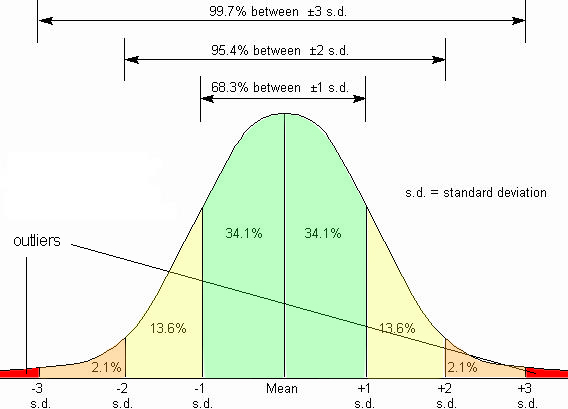
\includegraphics[width=0.65 \textwidth]{images/outlier_detection}
  \caption{\emph{Outlier detection} tramite gaussiana univariata}
  \label{fig:outlier_detection}
\end{figure}



\nocite{*}

\addcontentsline{toc}{section}{Riferimenti bibliografici}
\printbibliography
\end{document}  
